\documentclass[10pt,conference,blind]{IEEEtran}

\IEEEoverridecommandlockouts

% The preceding line is only needed to identify funding in the first footnote. If that is unneeded, please comment it out.

\usepackage{enumerate}
\usepackage{caption}
\usepackage{cite}
\usepackage{amsmath,amssymb,amsfonts}
\usepackage{algorithmic}
\usepackage{graphicx}
\usepackage{supertabular}
\usepackage{textcomp}
\usepackage{xcolor}
\usepackage{colortbl}
\def\BibTeX{{\rm B\kern-.05em{\sc i\kern-.025em b}\kern-.08em
    T\kern-.1667em\lower.7ex\hbox{E}\kern-.125emX}}
\usepackage{listings}
\usepackage{color}
\usepackage{scalefnt}
\usepackage{multirow}
\usepackage{pifont}
\usepackage{xspace}
\usepackage{todonotes}
\usepackage{booktabs}
\usepackage{longtable}
\usepackage{tabularx} 
\usepackage{multicol}
\usepackage{listings}
\usepackage{xspace}
\usepackage{booktabs}
\usepackage{siunitx}
\usepackage{amsmath,amssymb,amsfonts}
\usepackage{algorithmic}
\usepackage{graphicx}
\usepackage{graphics}
\usepackage{textcomp}
\usepackage{siunitx}
\usepackage{xcolor}
\usepackage{csquotes}
\usepackage{array}
\usepackage{listings}
\usepackage{color}
\usepackage{scalefnt}
\usepackage{multirow}
\usepackage{pifont}
% \usepackage{appendix}
\usepackage[framemethod=TikZ]{mdframed}
\definecolor{oldlace}{rgb}{0.99, 0.96, 0.9}
\newmdenv [ %
 skipabove=\topsep,
 skipbelow=\topsep,
 leftmargin       = 2,
 rightmargin      = 2,
 splittopskip     = \topskip]{mh}

\newmdenv [ %
 skipabove=\topsep,
 skipbelow=\topsep,
 roundcorner = 5pt,
 leftmargin = 2,
 rightmargin = 2,
 % backgroundcolor = oldlace,
 innertopmargin = 3,
 splittopskip = 3]{mq}

\definecolor{javared}{rgb}{0.6,0,0} % for strings
\definecolor{javagreen}{rgb}{0.25,0.5,0.35} % comments
\definecolor{javapurple}{rgb}{0.5,0,0.35} % keywords
\definecolor{javadocblue}{rgb}{0.25,0.35,0.75} % javadoc
\lstset{
  basicstyle=\footnotesize\tt,        % the size of the fonts that are used for the code
  breakatwhitespace=false,         % sets if automatic breaks should only happen at whitespace
  breaklines=true,                 % sets automatic line breaking
  captionpos=b,                    % sets the caption-position to bottom
  extendedchars=true,              % lets you use non-ASCII characters; for 8-bits encodings only, does not work with UTF-8
  frame=single,                    % adds a frame around the code
  language=Java,                 % the language of the code
  keywordstyle=\bf,
  showspaces=false,                % show spaces everywhere adding particular underscores; it overrides 'showstringspaces'
  showstringspaces=false,          % underline spaces within strings only
  showtabs=false,                  % show tabs within strings adding particular underscores
  tabsize=2,                       % sets default tabsize to 2 spaces
  keywordstyle=\color{javapurple}\bfseries,
  stringstyle=\color{javared},
  commentstyle=\color{javagreen},
  morecomment=[s][\color{javadocblue}]{/**}{*/},
  numbers=left,
  numberstyle=\tiny\color{black},
  stepnumber=1,
}    
\AtBeginDocument{%
  \providecommand\BibTeX{{%
    \normalfont B\kern-0.5em{\scshape i\kern-0.25em b}\kern-0.8em\TeX}}}

\newcommand{\clang}{C\nolinebreak\xspace}

\newcommand{\cpplang}{C\nolinebreak\hspace{-.05em}\raisebox{.4ex}{\small\bf +}\nolinebreak\hspace{-.10em}\raisebox{.4ex}{\small\bf +}\xspace}

% TODO: Completar
\newcommand{\minedprojects}{72\xspace}

\newcommand{\rb}[1]{\todo[inline]{{\bf (rb note) }#1}}
\newcommand{\diego}[1]{\todo[inline,color=green]{{\bf (diego note) }#1}}
\newcommand{\adriano}[1]{\todo[inline,color=yellow]{{\bf (adriano note) }#1}}
\newcommand{\castor}[1]{\todo[inline,color=pink]{{\bf (castor note) }#1}}

\newcommand{\rqa}{What is the impact of atoms of confusion on the comprehension of
  JavaScript code?}

\newcommand{\rqb}{Do JavaScript developers identify atoms of confusion as contributing to program misunderstanding?}

\newcommand{\rqc}{What are the particular JavaScript idioms and language constructs that might cause source code misunderstanding?}

\newcommand{\rqd}{What is the frequency of occurrence of atoms of confusion in practice (i.e., in open-source JavaScript projects)?}


\lstset{language=C}
\lstset{
 morekeywords={printf}
}

\newcommand{\lhs}{left-hand side\xspace}
\newcommand{\rhs}{right-hand side\xspace}

\lstdefinelanguage{JavaScript}[]{Java}{
  morekeywords={let, console.log},
  moredelim=[is][\textcolor{darkgray}]{\%\%}{\%\%},
  moredelim=[il][\textcolor{darkgray}]{§§}
}

\begin{document}
\newenvironment{atom}[1]
  {\mdfsetup{
    frametitle={\colorbox{white}{\space#1\space}},
    innertopmargin=10pt,
    frametitleaboveskip=-\ht\strutbox,
    frametitlealignment=\center
    }
  \begin{mdframed}%
  }
  {\end{mdframed}}

\title{On The Impact of Atoms of Confusion in JavaScript
Code}

\author{\IEEEauthorblockN{Anonymous}}


%% \author{\IEEEauthorblockN{1\textsuperscript{st} Given Name Surname}
%% \IEEEauthorblockA{\textit{dept. name of organization (of Aff.)} \\
%% \textit{name of organization (of Aff.)}\\
%% City, Country \\
%% email address or ORCID}
%% \and
%% \IEEEauthorblockN{2\textsuperscript{nd} Given Name Surname}
%% \IEEEauthorblockA{\textit{dept. name of organization (of Aff.)} \\
%% \textit{name of organization (of Aff.)}\\
%% City, Country \\
%% email address or ORCID}
%% \and
%% \IEEEauthorblockN{3\textsuperscript{rd} Given Name Surname}
%% \IEEEauthorblockA{\textit{dept. name of organization (of Aff.)} \\
%% \textit{name of organization (of Aff.)}\\
%% City, Country \\
%% email address or ORCID}
%% \and
%% \IEEEauthorblockN{4\textsuperscript{th} Given Name Surname}
%% \IEEEauthorblockA{\textit{dept. name of organization (of Aff.)} \\
%% \textit{name of organization (of Aff.)}\\
%% City, Country \\
%% email address or ORCID}
%% \and
%% \IEEEauthorblockN{5\textsuperscript{th} Given Name Surname}
%% \IEEEauthorblockA{\textit{dept. name of organization (of Aff.)} \\
%% \textit{name of organization (of Aff.)}\\
%% City, Country \\
%% email address or ORCID}
%% \and
%% \IEEEauthorblockN{6\textsuperscript{th} Given Name Surname}
%% \IEEEauthorblockA{\textit{dept. name of organization (of Aff.)} \\
%% \textit{name of organization (of Aff.)}\\
%% City, Country \\
%% email address or ORCID}
%% }

\maketitle

% Número das páginas. Remover para camera-ready
% útil para nós e Program Chair que pode ver o total de páginas facilmente
\thispagestyle{plain}
\pagestyle{plain}

\begin{abstract}
Evolving legacy code is a challenging task, particularly when the code has been poorly written---which imposes a significant cognitive load on developers when trying to familiarize themselves with a legacy codebase. Previous research has investigated the impact of small code patterns that contribute to misunderstanding the source code written in C and C++. However, little is known about the influence of these small code patterns (hereafter atoms of confusion) on understanding dynamic languages (such as JavaScript). In this work, we present the results of a mixed-method research: a survey, a set of interviews with practitioners, and a mining software repositories (MSR) effort.
Our goal is to investigate the impact of atoms of confusion on understanding JavaScript code---a dynamically typed language whose popularity is growing in the most different application domains (from web programming to backend and IOT development). From our survey and interviews, we confirm that atoms of confusion lead to code that is hard to understand: developers correctly predict the outcome of at least 15\% more cases when an atom of confusion is not present in 6 out of 9 atom candidates. Also, the results of our MSR effort reveal that atoms of confusion frequently arise in open-source JavaScript systems: the Comma Operator is present in 11\% of the projects in our dataset; while five other atom candidates
appear in more than 60\% of the projects---including the atoms Assignment as Value and Omitted Curly Braces, which appear in 8253 and 53357 times,
respectively. Our investigation also reveals additional JavaScript constructs and idioms that might hinder developers from understanding JavaScript code. For instance, even experienced JavaScript developers agree that it is hard to understand code that uses callback functions, even though we found widespread use of callbacks in our projects dataset. Altogether, our findings might help developers better understand the implications of atoms of confusion on understanding JavaScript code and contribute to the design of new program transformation tools that aim to simplify JavaScript code.
\end{abstract}

\begin{IEEEkeywords}
datasets, neural networks, gaze detection, text tagging
\end{IEEEkeywords}

\section{Introduction}
\label{intro}

% The source code of a program can be naively understood as a collection of sentences in a language that would be interpreted by a computer (or compiled into a lower level representation and then executed by a computer). Nonetheless, this understanding is far from being complete. While it is not possible to execute programs without writing them in a way that the machine is able to interpret, it is also very difficult to develop software that performs complex tasks if developers do not care about how easily other programmers are going to understand its source code \cite{DBLP:journals/cj/Knuth84}.

% \rb{acho que esse proximo paragrafo pode ser excluido}
% \diego{também acho}

% {\color{blue}That means programming should, in various ways, be regarded as an act of communication. In this context, the programmer is often faced with a dilemma. When initially confronted with a problem they have to solve, the programmer will proceed to employ their cognition into developing the logic of the solution, whilst simultaneously having to worry about writing ``syntactically correct'' code for the machine to parse and translate. The problem is that, during the time spent solving the problem and communicating with the computer, developers often do not have enough cognitive resources to also make considerations about whether their code is understandable by other programmers. Therefore, it takes a change of track to make the code easier to understand \cite{DBLP:books/daglib/0019908}. Not proceeding with such change of track is one of the reasons why ``confusing'' language constructs and idioms arise and remain in a program.}

Source code misunderstandings can occur due to diverse reasons.
A poorly understood requirement might lead to poorly implemented code.
An intricate algorithm may require extra time to be fully comprehended.
Nevertheless, programming languages can also be at fault.
Specific syntax and semantics of a language can cause misunderstandings. The same applies to some code idioms and stylistic choices~\cite{DBLP:conf/msr/GopsteinZFC18}.

% \diego{acho que o prox. parágrafo deve ser adaptado ou até removido}
% {\color{blue}A direct consequence of the presence of these idioms in the code base is that it becomes even more difficult to develop new features for the software. 
% According to Gopstein et al. \cite{DBLP:conf/sigsoft/GopsteinIYDZYC17} ``\emph{the ability to understand pre-existing source code is one of the most important elements of a continuously successful software project}'', it follows that, if one cannot properly understand the \emph{purpose} and \emph{meaning} of a piece of code, they are not going to be able to build upon its existing parts.
% Other consequences of the presence of confusing code include: 
% (a) increased probability of bug introduction, due to a lack of proper understanding of what the program does; 
% and (b) loss of internal quality measures, such as cohesion and coupling. 
% This phenomenon usually leads to an architectural erosion. 
% All these situations, which usually compound each other, expose the necessity of developing recommendations, tools, and techniques that help developers to avoid writing confusing code, identify potentially confusing code, and transform confusing code into clear code. 
% Therefore, it is necessary to understand what programming language constructs and idioms might lead to code that is hard to understand.}

JavaScript is the most widely used language for web development and the most often adopted language on GitHub~\cite{BugsJS:ICST}. At the same time, JavaScript is infamously known to be ``the worst most popular language in the world''\footnote{https://github.com/getify/You-Dont-Know-JS/blob/2nd-ed/preface.md}. It is a weakly typed language~\cite{DynamicBehaviorJS:PLDI} that provides object-oriented, functional, and imperative constructs~\cite{JS-CodeSmells:SCAM}, in addition to features such as run-time evaluation~\cite{BugsJS:ICST,ClientSideBugsJS:TSE}, and asynchronous operations. All these 
%diverse characteristics and capabilities
features combined make JavaScript source code fertile ground for errors~\cite{BugsJS:ICST,ClientSideBugsJS:TSE} and confusion~\cite{JSGoodParts:book}.

Our research aims to help practitioners identify potentially confusing snippets of code, so that
developers could replace them with clearer code.
To achieve that, we investigate {\color{red}XYZ} JavaScript idioms that
might compromise program understanding. These idioms correspond to a set of candidates for \emph{atoms of confusion} in
JavaScript---that is, small
pieces of code that hinder developers' understanding of the source code of a program
for which there are functionally equivalent alternatives that are easier
to understand~\cite{DBLP:conf/sigsoft/GopsteinIYDZYC17}. For instance, consider
the pair of code snippets in Listing~\ref{fig:lst01} (adapted from \textsc{NervJS/taro}
for presentation purpose only). The code in the left of the figure contains two atoms of confusion discussed in a previous work~\cite{DBLP:conf/sigsoft/GopsteinIYDZYC17}: \emph{Logic as Control Flow} and \emph{Post-increment}. On the right we present a cleaned version of the code, that is, without atoms of confusion. According to
Gopstein et al.~\cite{DBLP:conf/sigsoft/GopsteinIYDZYC17} removing
the atom \emph{Logic as Control Flow} and \emph{Post-increment} improves the accuracy of
program understanding tasks in  41\% and 34\%, respectively.

Among the atoms in this work, X are shared between JavaScript and \clang/\cpplang (e.g., pre/post-increment), while Y others are specific to JavaScript, e.g., the atom Assignment as Value.
Recent work~\cite{DBLP:journals/ese/MedeirosLAAKRG19,DBLP:conf/sigsoft/GopsteinIYDZYC17} has
already explored the impact of atoms of confusion on program understanding,
and confirmed they negatively impact source code understandability.
However, they were constrained to statically typed languages (e.g., \clang and \cpplang).
To the best of our knowledge, we are the first to explore atoms of confusion
in the context of a dynamically typed language (JavaScript).\castor{Review the number of atoms, X, and Y.}

\begin{figure*}[thb]
\noindent\begin{minipage}{.45\textwidth}  
\begin{lstlisting}[language=JavaScript]
res = properties.reduce((s, b) => {
  b && s++
  return s
}
\end{lstlisting}
\end{minipage}\hfill
\begin{minipage}{.45\textwidth}
\begin{lstlisting}[language=JavaScript]
res = properties.reduce((s, b) => {
  if(b) {
    s = s + 1
  }
  return s
}
\end{lstlisting}
\end{minipage}
\label{fig:lst01}
\captionof{lstlisting}{Code snippet from \textsc{NervJS/taro} project. Line 2 in the left hand side of the figure contains two
  atoms of confusion discussed in ~\cite{DBLP:conf/sigsoft/GopsteinIYDZYC17}: \emph{Logic
  as Control Flow} and \emph{Post-increment}. In the right hand side, we present the alternative code without atoms of confusion. We could simplify the code on the left even more, by using \texttt{filter} and \texttt{length} instead of the \texttt{reduce} recursive pattern (e.g., \texttt{res = properties.filter(p => p).length}).}
\end{figure*}

To understand whether an atom of confusion introduces misunderstandings, we surveyed 140 developers from the Reddit community. Their task was to predict the output of short snippets of code, with half of them containing atoms of confusion. We found an improvement of at least 15\% in the correct answers when removing the confusing code for seven atoms (out of 9 atoms). The presence of the Comma Operator atom, for instance, can increase the average time to predict the output by 65\%, while the behavior of snippets containing the Pre-Increment atom were predicted 44\% faster.  An atom's presence---or lack of---in open-source repositories may reveal cases where developers should be more or less careful when writing code. To identify such cases, we mined the 100 most popular JavaScript projects from GitHub and found a total of X atoms in the analyzed projects. To learn more about the misunderstandings in the snippets used in the survey, we interviewed 15 experienced professional developers. Participants preferred code snippets \textit{without} an atom in 70\% of the cases, therefore corroborating to the survey findings. During the MSR and interview studies, we also explored additional atom candidates that are specific to the
JavaScript language. 


Altogether, the main contributions of this paper are:
\rb{revisar as contribuicoes quando o artigo estiver mais maduro. por enquanto, vamos ignorar esses bullets.}

\begin{itemize}
    \item A study about the impact of atoms of confusion on a
    dynamic language.
    \item A list of additional atoms of confusion addressing particular 
    JavaScript constructs and idioms.
    \item A library and infrastructure to mine atoms of confusion using 
    code queries (implemented in the .QL language). This library and 
    infrastructure are freely available and might help researchers and 
    practitioners to automate program analysis at a large scale.
\end{itemize}



% Our research aims to identify and characterize JavaScript \textit{atoms of confusion}: small pieces of code that hinder developers' understanding of the source code of a program~\cite{DBLP:conf/sigsoft/GopsteinIYDZYC17}.
% Previous research has confirmed the negative impact of atoms of confusion when considering statically typed languages (e.g., \clang and \cpplang)~\cite{DBLP:journals/ese/MedeirosLAAKRG19, DBLP:conf/msr/GopsteinZFC18}.

% Recent works have explored the impact of \emph{atoms of confusion}~\cite{DBLP:journals/ese/MedeirosLAAKRG19,DBLP:conf/sigsoft/He19,DBLP:conf/msr/GopsteinZFC18} on program understanding.
% Atoms of confusion correspond to small pieces of code that hinder developers' understanding of the source code of a program. 
% Previous research has confirmed the negative impact of atoms of confusion when considering statically typed languages (e.g., \clang and \cpplang)~\cite{DBLP:journals/ese/MedeirosLAAKRG19,DBLP:conf/msr/GopsteinZFC18}.

% In this work, to the best of our knowledge, we are the first to explore this issue in the context of a dynamically typed language (JavaScript), answering the following research questions:
% \emph{How do JavaScript developers  identify atoms of confusion as contributing to program misunderstanding?}
% \emph{What is the impact of atoms of confusion on misunderstanding JavaScript code?},
% and \emph{What is the frequency of occurrence of  atoms of confusion in practice?} 
% To answer these research questions, we conduct this investigation using a mixed-methods approach, involving a survey, a set of interviews, and an activity of mining source code repositories. Altogether, the main contributions of this paper are

% \rb{revisar as contribuicoes quando o artigo estiver mais maduro. por enquanto, vamos ignorar esses bullets.}

% \begin{itemize}
%     \item A first study about the impact of atoms of confusion on a
%     dynamic language. {\color{red}present some of the results here.}
%     \item A library and infrastructure to mine atoms of confusion using 
%     code queries (implemented in the .QL language). This library and 
%     infrastructure is freely available and might help other researcher and 
%     practitioners to automate program analysis at a large scale. 
%     \item A list of additional atoms of confusion addressing particular 
%     JavaScript constructs and idioms. {\color{red}present some insights 
%     about these additional atoms here}
% \end{itemize}

\section{Background and Related Work}
\label{back}
\subsection{Program Comprehension}\castor{It would be nice to have a table with the atom candidates similar to the one that appears in Gopstein et al. 2017.}

The concept of program comprehension is central to software maintenance and feature development \cite{DBLP:conf/iwpc/TilleySP96}. Regardless of whether they are performing maintenance on legacy software or adding new features, programmers have to understand what the source code does before making any improvements. A natural consequence of this is that a programmer must also have in mind that other programmers (or their future selves) 
%are going to have to
will
spend time trying to understand the code being currently developed before doing any work themselves.

As program comprehension is regarded less as a systematic process than as an objective \cite{DBLP:journals/ibmsj/OHareT94}, there is no single approach or framework that is capable of yielding easily understandable programs. Factors such as problem domain, size and complexity of the code base, and available tools all vary significantly between different working settings. These aspects, combined with differences between individuals, which can include experience, working memory capacity, and other cognitive traits, make it clear that program comprehension should be approached in different ways in different contexts. 

However, one of the ways in which programs become less comprehensible occurs when programmers favor complicated syntactic constructs instead of using semantically equivalent versions---when these exist---allowed by the language or framework they are working with. Although this can be, to an extent, a personal matter, since different individuals might hold different opinions on whether a given syntax is difficult to understand, it is possible to empirically investigate if there exist programming languages' constructs or idioms that are considerably harder to understand, leading readers of the code to frequently make incorrect predictions of its behavior. 

\subsection{Atoms of Confusion}\label{sec:aoc}

The concept of atoms of confusion was introduced by Gopstein et al. \cite{DBLP:conf/msr/GopsteinZFC18}, who defined them as small code patterns that can verifiably lead to misunderstandings. In addition, for a code pattern to be considered an atom, there must be some alternative pattern or language construct that is functionally equivalent and less likely to cause confusion. Their work laid an empirical framework to identify such atoms. In summary, the basic approach to determine whether a code pattern is an atom involves: (i) identifying a set of atom candidates; (ii) identifying alternative constructs to these atom candidates; (iii) building a set of small programs that each contain a single atom candidate; (iv) building different versions of these programs where the atoms were removed and which employ the aforementioned alternative constructs; (v) in an experiment or semi-experiment, presenting subjects with the two versions of the programs for each atom candidate and asking subjects to predict their outputs; (vi) statistically comparing the performance of the subjects.
%By having subjects evaluate code where in the expected output relied exclusively on evaluating the result of previously known confusing programs that had been written in \clang or \cpplang, and asking the participants to predict the output of a set of code snippets where the atoms had been removed, the authors were able to isolate and measure the impact of such confusing atoms. 

One main example that occurs in many programming languages is the Change of Literal Encoding. For instance, the \clang code statement \lstinline{printf("\%d", 013);} 
often leads programmers to predict the output to be \texttt{13}, even though the correct answer is \texttt{11}. This occurs because a leading \texttt{0} in a number literal indicates that the number is in base \texttt{8}, a fact that is not only unknown to less experienced programmers, but misleading even for seasoned developers. After formulating a list of 19 potential atoms, Gopstein et al. \cite{DBLP:conf/sigsoft/GopsteinIYDZYC17} were able to identify 15 snippets that present a statistically significant difference in comparative answer correctness when each of the 15 atoms was removed. The least confusing atom showed a 14\% boost in prediction accuracy when the atom was removed, whereas the most confusing one showed a 60\% accuracy increase. Our first study follows the empirical framework discussed in~\cite{DBLP:conf/sigsoft/GopsteinIYDZYC17}, for all atoms that have a counterpart in JavaScript. Gopstein et al. \cite{DBLP:conf/msr/GopsteinZFC18} also performed a qualitative analysis on the different nature of confusion amongst the atoms, noting that, for some atoms, a particular incorrect answer was prevalent, whilst there was a distribution of incorrect ones in other atoms. 

The work of Gopstein et al. \cite{DBLP:conf/sigsoft/GopsteinIYDZYC17} presented the results of comprehensive research on atoms of confusion that can be found in the \clang and \cpplang~languages. Even though JavaScript is a dynamic language that differs from \clang in a variety of aspects, it also has a number of constructs in common. In addition, the imperative aspects of the language are syntactically similar to \clang, e.g., assignments, conditional expressions, \texttt{if}-statements, pre and post increments and decrements, among others. On the one hand, this means that some of the atoms of confusion that exist in \clang programs may also occur in JavaScript code. On the other hand, differences between the languages and the surrounding programming cultures may lead to code patterns that are atoms of confusion in one language not being atoms in the other one.  
%Although JavaScript allows us to program in different paradigms from the one C follows, most of the JavaScript code found in popular repositories are written under the imperative paradigm. Also, both languages share many syntactical rules, which allows us to replicate some of the C atoms in JavaScript.

Medeiros et al. \cite{DBLP:journals/ese/MedeirosLAAKRG19} analyzed 50 open source projects written in the C language with the goal of evaluating 12 code patterns called ``misunderstanding patterns'' by the authors. Many of these misunderstanding patterns are either atoms of confusion or atom candidates~\cite{DBLP:conf/sigsoft/GopsteinIYDZYC17}. This study shows that these patterns are prevalent; among these 50 projects, there are more than 109K occurrences of misunderstanding patterns. 
In order to gauge the relevance of these misunderstanding patterns, the authors sent 35 pull requests removing occurrences of these patterns to randomly-selected open source projects. The authors of the study received feedback for 21 of these pull requests and the maintainers of the projects accepted 8 of them (22.86\%). The authors also analyzed 36 coding style guides from these projects, but found few guidelines specifically addressing misunderstanding patterns. 

% Para compreender a relevância desses misunderstanding patterns os autores enviaram 35 pull requests selecionados aleatoriamente, para remover as ocorrências desses padrões encontrados no código dos projetos avaliados. Os autores receberam feedback para 21 pull requests, e os desenvolvedores aceitaram 8 pull requests (38\%). Os autores também analisaram 36 Guidelines dos open-source projects provide for developers regarding misunderstanding code patterns.

Castor~\cite{castor2018} presented a preliminary catalog of six atom candidates for the Swift programming language. Unlike JavaScript, in Swift most of the atoms identified by Gopstein et al.~\cite{DBLP:conf/sigsoft/GopsteinIYDZYC17} are avoided by construction, e.g., it does not have assignments as values, increment operators, or macros. The paper also presents a structured definition for what it means for a code pattern to be an atom of confusion and a set of general principles to help in the identification of new atoms. 

%Castor \cite{castor2018} apresentou um catalógo preliminar de átomos de confusão na linguagem de programação Swift. O autor identificou 6 estruturas candidatas a átomos de confusão em Swift. Foram omitidos os candidatos que tinham uma correspondência direta com os átomos previamente identificados por Gopstein et al. \cite{DBLP:conf/sigsoft/GopsteinIYDZYC17}.

According to Arnaoudova et al.~\cite{Arnaoudova:2016:LAW}, Linguistic Antipatterns (LA) are \textit{``recurring poor practices in the naming, documentation, and choice of identifiers in the implementation of an entity [..] that may impair program understanding''}. These antipatterns are design issues that go against developer's  intuition about a program, for example, a \texttt{set} method that returns a result. Similarly to atoms of confusion, LAs occur at the source code level and hinder code readability. Differently from atoms of confusion, LAs are more akin to design principles than code idioms. In addition, they are language-agnostic, unlike atoms of confusion.

Santos and Gerosa~\cite{Santos:2018:ICP} analyze the impact of eleven coding practices on program readability. Some of them, such as avoiding more than three levels of code
block nesting, are atom candidates. 
% Diego: Troquei "this work" para "their work". Removi o "more" de "are more related"
Their work evaluates the coding practices solely based on personal opinions of the study subjects. Furthermore, it focuses on the Java language. Finally, most of the practices are related to code formatting than language constructs or idioms.

%% \castor{Provavelmente devemos reduzir o espaço tomado pelos quatro trabalhos acima, a depender da existência de outros. O de Linguistic Antipatterns talvez até devesse sair.}
%% \rb{Incluir os trabalhos do grupo do Marcio Ribeiro e do Fernando Castor. Quais outros trabalhos deveriamos incluir aqui?}

\section{Study Settings}
\label{method}

The main goal of this research is to investigate the impact of atoms of confusion in JavaScript code comprehension. As such, in this paper we answer the following research questions: 

\begin{enumerate}[(RQ1)]
    \item Do JavaScript developers identify atoms of confusion as contributing to program misunderstanding? 
    \item What is the impact of atoms of confusion on the comprehension of JavaScript code? 
    \item What are the particular JavaScript idioms and language constructs that might cause source code misunderstanding?
    \item What is the frequency of occurrence of atoms of confusion in practice (i.e., in open-source JavaScript projects)?
\end{enumerate}

 
Answering these research questions has several implications. For instance, we can either generalize or refute the perceptions about atoms of confusion already discussed in the literature (goal of research questions (RQ1) and (RQ2)). In addition, answers to the third and fourth questions allow us to enrich existing catalogs about atoms of confusion and discuss how often they occur in practice. Our motivation to detect the presence and impact of atoms of confusion is also motivated by the possibility of laying the foundations for the implementation of libraries that can automatically transform code into its cleaner versions---though we postpone these results to a future research work. This might lead to a new catalog of refactoring for removing atoms of confusion.  To answer these research questions we conduct a mixed-methods study, including a survey, a set of interviews, and an effort of mining JavaScript software repositories.  


 \subsection{First Study: Survey}\label{sec:survey-settings}\castor{Eu mudaria os títulos desta sub-seção e das duas próximas para "First study: Survey", "Second study: Mining open source repositories", etc. Vale a pena manter "First study", etc.?}
% \subsubsection{The Atoms Considered In This Work}

In the first study, our goal was to collect evidence to answer two specific questions: 
\begin{itemize}
    \item \emph{Do code snippets that contain atoms of confusion produce a higher misunderstanding rate when programmers try to predict their outcome?}
    \item \emph{Do code snippets with atoms of confusion require programmers to take longer to predict their output?}
\end{itemize}

To address these questions we conducted a survey to assess the impact of atoms of confusion on understanding JavaScript code. Since JavaScript and C have some constructs in common (Section~\ref{sec:aoc}), we first selected a set of atoms of confusion for the \clang language~\cite{DBLP:conf/sigsoft/GopsteinIYDZYC17} that may also exist in JavaScript programs. {\color{red}In addition, we consider a particular atom that is exclusive to JavaScript in this first study}. Appendix~\ref{sec:appendix-atoms} summarizes all atoms we consider in our research. 

\subsubsection{Survey design} 

The design of our first study aims to block two variables (developer experience and the code snippets) and considers two treatments: the presence or absence of 
atoms of confusion within the code snippets. 
To achieve such a design goal, controlling the effect of experience and individual code snippets, we resorted to the \textit{Latin Square Design} \cite{Hunter-Experimenters}. Using this design we create a 2 x 2 matrix in which each row represents a subject and each column indicates the set of code snippets. The design of each square (a replica) is such that no treatment is repeated in the same row or column. For example, if a given subject (P1) is asked to predict the output of code snippets that contain atom candidates \texttt{\{1,2,3,4,5\}}, then, when answering questions about non-confusing code snippets, they will only be presented with non-confusing versions of atom candidates \texttt{\{6,7,8,9,10\}}. Furthermore, a given subject (P2), which constitutes the second row of our example square, will be asked questions about the non-confusing versions of \texttt{\{1,2,3,4,5\}}, and will answer questions about confusing snippets of \texttt{\{6,7,8,9,10\}}. By doing that, we guarantee that all of our 20 snippets are contained within each square, and that each configuration occurs only once within a square. Figure \ref{fig:latinsquare} offers a visual representation of the concept.

  \begin{figure}[htb!]
      \noindent
      \centering
      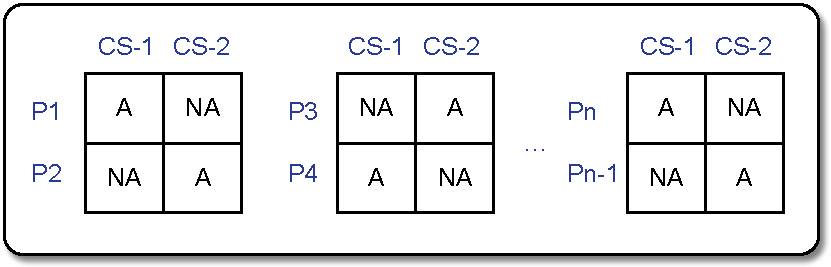
\includegraphics[scale=.50]{images/latin-square.pdf}
      \caption{Latin square design. Each ``square'' corresponds to 
      a replica in our study. Each replica comprises two students (square rows) 
      and two sets of code snippets (CS-1 and CS-2). We randomly apply the 
      treatments (atom or non-atom code) to the cells of the squares.} 
      \label{fig:latinsquare}
  \end{figure}


Having selected 10 atoms in our first study, we wrote small pieces of code that contained each atom. We also wrote their equivalent snippet without the confusing idioms and constructs, leading to a total of 20 code snippets. In order to reduce the cognitive effort, we decided that each subject would be asked to predict the output of a subset of 10 listings, wherein each subset contained 5 blocks that contained atoms of confusion, whilst the remaining 5 had the atoms removed. The order in which the questions were presented was randomized. By doing this, we were seeking to minimize the chances of subjects being aware that the current listing they were analyzing contained (or not) atoms of confusion.
That is, each respondent of the survey should indicate what would be the outcomes of the code snippets, some of them having atoms of confusion (while other code snippets did not). 
We measured answer correctness and total time each participant needed to answer reach question of their survey. 

\subsubsection{Survey Instrument} 

We implemented our survey as a web application. As part of this 
effort, we carried out an informal pilot whose main objectives were: to spot bugs in the application and in the data collection mechanism; to gain feedback from respondents about the user experience of the application; and to formulate an estimate about how long answering the survey would, on average, take. Fellow undergraduate students, professional colleagues, and friends took the pilot survey. Some users reported layout defects, and many reported that the landing page did not explain the survey well enough. We also spotted minor issues with our routines to create and populate the Latin Squares. 

We organized the survey in {\color{red}three} sections. The first section aims to characterize the subjects, asking for their age, education level, and programming experience. We also included a check button, whose checking meant users agreed that all collected data would be used solely for research purposes. In the second section, we presented to the participants a small set of instructions, where we explained how the survey worked and asked them to dedicate their attention to it. We stressed to participants the importance of not using any aids during the survey, such as online or console interpreters. For each question page, we kept track of whether or not the subjects switched windows. 

The next section of the survey presented a sequence of 10 questions, each containing a code snippet. For each question, there was a text box where the answer should be written. There was also an ``I do not know'' button, which, when clicked, led the subject to the next question. In our setting, ``I do not know'' was treated as a wrong answer. The code snippets were presented as images copied from a text editor, so as to demotivate respondents from resorting to external resources by copying and pasting the code into an interpreter. Upon submitting their answer for a particular question, the subject was automatically led to a similar page, containing another snippet.
    
We decided not to provide feedback about the time students took to answer each question. Nor did we tell them whether their answers were correct or not. Our main concern was to avoid introducing bias for future respondents. Since we posted the survey in a social media platform, if we gave respondents instant feedback, they might post comments on particular atoms, therefore interfering with future participants' thought process.

% \rb{nao acho esse paragrafo necessario} 
% \adriano{o de baixo ne? eu tambem acho}

% As we mentioned before, we first wrote the code listings in a text editor, and took pictures of it. In the case of an atom of confusion that was exclusive to JavaScript, which we called \textit{Automatic Semicolon Insertion} (see Appendix~\ref{sec:appendix-atoms}), it was necessary to remove the syntax highlighter. Even though semicolons at the end of statements are optional to programmers in JavaScript, the interpreter automatically inserts them into the code. Our text editor was incorrectly highlighting a line break after a return statement, even thought it was valid JavaScript syntax. We had thus to turn the highlighter off to take the picture of this atom. 

\subsubsection{Survey audience}

\diego{Esses detalhes são possíveis candidatos para remoção, se precisarmos de espaço}
{\color{blue}We invited developers to answer our survey by sending invitations to communities of JavaScript programmers on the Internet. Our initial plan was to try to engage contributors for two major JavaScript projects, namely Node.js and NPM. None of the projects, though, offered a direct way to interact with the community, such as an online discussion forums or mailing list. We would be required to first make contact with the projects' leaders, and only then would we have a chance to approach potential respondents. Due to time constraints, we decided to look for respondents elsewhere.}
We then posted the survey on Reddit.\footnote{Reddit is a North American online discussion platform. Its discussion threads, often called subreddits, are sorted by subject. For our research, we posted information and links to the survey in two JavaScript subreddits.}. We explained our research purposes, and asked developers of any level of expertise to take the survey. To incentivize serious engagement, we proposed to raffle \$50 gift cards on Amazon products at the end of the survey. Within twelve hours we collected more than 150 answers, populating more than 70 replicas of the Latin Squares. We were able to collect significant data on time taken and discrepancies in answer correctness between confusing and non-confusing versions of the snippets. 
    
\rb{acho que podemos mover esse proximo paragrafo para a secao de resultados, ou de ameacas}
\adriano{acho que pode ir para resultados. nao considero uma ameaca pois eu e o Caio tratamos manualmente as entradas a serem removidas e garantimos a integridade dos latin squares}

Inconsistencies may arise when each square is being built. The main source of inconsistency we faced was when a user quit in the middle of the survey. When this happened, his row in the square was left incomplete. We considered all squares which contained incomplete rows to be invalid, and discarded them. Since we had a large enough number of samples, the squares we had to discard did not impact our results.
    
    
% \subsubsection{Pilot Survey}    

% To validate the web application we developed to conduct the survey, we ran an informal pilot survey whose main objectives were:
%     \begin{itemize}
%         \item To spot bugs in the application and in the data collection mechanism;
%         \item To gain feedback from respondents about the user experience of the application;
%         \item To formulate an estimate about how long the survey would, on average, take.
%     \end{itemize}
    
% We had fellow undergraduate students, work colleagues and friends take the pilot survey. We discovered that the aspect that needed most improvement was the user experience. Some users reported layout defects, and many reported that the landing page did not explain the survey well enough. We also spotted minor issues with our routines to create and populate the Latin Squares. After performing all the necessary changes, we were ready to conduct another experiment.

\rb{Comentei o survey com alunos}

% \subsubsection{A Survey With Undergraduate Students}
%     Our second attempt was due to courtesy of a professor of our department. During the semester of the writing of this text, he was lecturing a Data Structures course, which is usually taken during the second semester of the undergraduate course. The professor agreed to take the students to a laboratory during one of his classes, and all the students who attended that day took the survey.
    
%     No issues were reported with the web application, and all answers were appropriately collected. This time, all the Latin Squares were being populated correctly, making the data we collected eligible for use in the final analysis. However, we opted to dispose of all the data we gathered in this occasion. What motivated this decision were the two following aspects:
%     \begin{enumerate}
%         \item The students were not focusing hard enough. Most students were not very serious about the survey. While we watched them answer the questions, we could see many students peeking at each other's screens. We could also clearly see students not taking nearly enough time to reason about the code, and answering the questions without giving it proper thought.
%         \item We needed a more diverse spectrum of respondents. In the beginning of our research, we established that we would need at least 25 Latin Squares in order to be able to have significant results. By conducting this survey, we were able to populate 11 Latin Squares. Compounded by the problem reported above, we were concerned that our spectrum of respondents might end up skewed towards undergraduate students with little or no JavaScript programming experience.
%     \end{enumerate}
    
%     These two facts led us to conclude we needed to conduct a survey in which partakers engaged voluntarily, whilst also having an incentive to think hard enough about the problems they faced. To address these points, we prepared our final setting.
    
\subsection{Second Study: Mining Software Repositories}

To understand how often atoms of confusion appear in real settings, and thus answer our fourth research question (\emph{What is the frequency of occurrence of atoms of confusion in practice?}), we mined a set of GitHub open source repositories. To this end, we first collected the most popular GitHub repositories that are primarily written is JavaScript. We measured popularity using the project's stargazers, and selected only projects with stargazers\_count > 100. This metric, available on  GitHub API, represents the number of stars a project received from users of the platform. The same metric has been used in a number of previous studies as a proxy to estimate project's popularity~\cite{gyimesi2019bugsjs}.

After filtering out JavaScript project candidates, in the second step we built a curate dataset comprising the top 100 most popular repositories. Examples of projects in this dataset include \textsc{React}, \textsc{Node JS}, and \textsc{AngularJS}. Table~\ref{tab:projects-statistics} presents some statistics about the projects we consider in our research. The size of the projects range from small ones (883 liens of code) to complex systems with more than 10 MLOC. All projects in our dataset have at least \num{1161} forks and \num{23643} stars. We automated all the steps to filter, clone, and collect the statistics from the repositories using Python scripts.

In the third step we mined atoms of confusion from the repositories in our curate dataset. We written source code queries usng the CodeQL language~\cite{moor:gttse2007}, in order to filter the atoms of confusion. CodeQL is an object-oriented variant of the Datalog language~\cite{rodriguez2020efficient}, and currently supports researchers and practitioners to query the source code of systems written in different languages (such as Java and JavaScript). 
We also automate the process of running the queries and exporting the results to a format that simplifies our analysis and the reproduction of this study. In the final step we carry out basic descriptive statistics, in order to understand how often the atoms of confusion appear in practice. 

\begin{table*}[ht]
 \centering
 \begin{tabular}{rrrrrrr}
   \hline
             & Min. & 1st Qu. & Median & Mean & 3rd Qu. & Max. \\ \hline
 Lines of Code           & \num{883}  & \num{14939} & \num{39520} & \num{281088.46} & \num{145990.75} & \num{10149685} \\
 Num. of Contributors    & \num{6}   & \num{121} & \num{243} & \num{431.82} & \num{436.75} & \num{4042} \\
 Num. of Forks           & \num{1161}   & \num{3365} & \num{5711} & \num{8201.96} & \num{8438.25} & \num{68826} \\
 Num. of Stars        & \num{23643} & \num{27542.25} & \num{35687.5} & \num{45284.86} & \num{47963.25} & \num{310725} \\
    \hline
 \end{tabular}
 \caption{Some descriptive statistics about the projects used in the study}
 \label{tab:projects-statistics} 
 \end{table*}
 
\subsection{Third Study: Interviews with Practitioners}

To complement our initial survey, we performed semi-structured interviews with professional JavaScript developers, aiming to identify their perceptions regarding code snippets containing atoms of confusion. We also asked each participant if they knew of any other JavaScript-specific construct that they regarded as confusing. In this section we details the protocol we followed to conduct the interviews, and we also describe how their results were analysed.

% Nós realizamos entrevistas semi-estruturas com o objetivo de identificar a percepção dos desenvolvedores com experiência em JavaScript sobre algumas questões relacionadas à compreensão de código em JavaScript. Assim, nesta Seção nós descrevemos os procedimentos adotados para selecionar os participantes para as entrevistas e detalhamos como as entrevistas foram conduzidas. Além disso, detalhamos como os resultados das entrevistas foram analisados.

\subsubsection{Participants Selection}: The participants of the interviews were invited personally by the authors, and the pool of potential participants was based on our network of contacts. Our main criterion of selection was that all participants had to be working professionally with JavaScript. We invited a total of 17 developers, and 15 of these agreed to participate, and throughout a two week period, we conducted all the interviews.

% Os participantes das entrevistas foram selecionados a partir da nossa rede de contatos. Nós convidamos 17 pessoas e 2 não responderam ao nosso convite para participar das entrevistas. Durante 2 semanas, nós entrevistamos 15 desenvolvedores. Iniciamente nós conduzimos duas entrevistas como piloto. Após o piloto com dois desenvolvedores com mais de 03 anos de experiência, nós adicionamos uma nova pergunta na entrevista: Você conhece alguma construção em JavaScript que leve a um mal entendimento do código? Ao finalizar as entrevistas, nós perguntamos ao desenvolvedor se ele conhecia algum outro desenvolvedor com experiência em JavaScript que pudesse nos indicar para participar das entrevistas. Nós entrevistamos 02 desenvolvedores a partir da indicação dos entrevistados. A Tabela \ref{pinterview} apresenta o perfil dos 15 participantes das entrevistas.

\subsubsection{Interview Process}

We conducted semi-structured interviews using a web conferencing software. All the interviews were recorded with the consent of participants. On average, the interviews lasted 26.29 minutes, with the shortest one lasting 14.59 minutes, and the longest one 43.06 minutes. The main goal of the interviews was to have developers assess in real time whether two versions of code with the same behavior differed in readability, and, if so, which version they regarded as the easier one to understand. The interviews were conducted by two of the authors of this text, and a third one listened to all the recordings to cross-validate the collected data.

% Nós conduzimos entrevistas semi-estruturadas utilizando um software de conferência de audio/video. Todas as entrevistas foram gravadas com o consenso dos entrevistados. As entrevistas tiveram uma duração de aproximadamente 26.29 minutos. A entrevista com menor duração foi de 14.59 minutos e de maior duração foi de 43.06 minutos. O objetivo ao realizar as entrevistas era identificar quais as construções em JavaScript podem corresponder a confusões de código. As entrevistas foram realizadas por dois dos autores deste artigo.

The interviews had three main parts. In the first one, we asked the developers the following demographic information: name, email, gender, level of education, current job position, JavaScript experience and other programming languages they have worked with. Table \ref{pinterview} presents the profile of each participant.

\begin{table*}[htb!]
\centering
\begin{tabular}
{|p{0.4cm}|p{0.9cm}|p{2.0cm}|p{7.0cm}|p{1.9cm}|p{3.0cm}|}
\hline
ID & Gender & Level & Role & JS Experience & Other Languages \\ \hline  
P1 & Male & Graduate & Developer at Federal Court of Accounts - TCU Brazil & 9 years & Java, PHP, C, Go  
\\ \hline
P2 & Male & High School & Developer at Luma Health & 3.5 years & Python, Go, Dart, Lua, C++, C\#
\\ \hline
P3 & Male & Graduate & Developer at Superior Labour Court - TST Brazil & 4 years & Java, C
\\ \hline
P4 & Male & Undergraduate & Developer at Brazilian Association of Research and Industrial Innovation - EMBRAPII & 3 years & Python, C, C++, Java, Go
\\ \hline
P5 & Male & Master Student & Developer na Qubo Technology & 3 years & Python, SQL
\\ \hline
P6 & Male & Graduate & Software Architect at Superior Labour Court - TST Brazil & >15 years & Java, PHP, C, Python , Ruby, C\# and R
\\ \hline
P7 & Male & Graduate & Developer na Stefanini & 6 years & C, C++, Java, Assembly, Kotlin
\\ \hline
P8 & Male & PhD & Developer Regional Labour Court - TRT Goiás, Brazil & 2 years & Java, Python
\\ \hline
P9 & Male & Graduate & IT Analyst at Regional Bank of Brasilia - BRB Brazil & 5 years & PHP
\\ \hline
P10 & Male & Master Student & Business Analyst and Developer at National Confederation of Industry - CNI Brazil & 4 years & Java, C\# and Python
\\ \hline
P11 & Male & Master Student & Software Architect at the University of Brasilia's Informatics Centre & 4 years & Java, Erlang, C\#, Cobol
\\ \hline
P12 & Female & Master & Software Engineers at Novatics & 1 year & C
\\ \hline
P13 & Male & Master & Developer at the Military Police of the Federal District - PMDF Brazil & 13 years & Java, PHP
\\ \hline
P14 & Female & Master Student & Developer at Neoway & 3 years & C, Python, Ruby
\\ \hline
P15 & Female &  Graduate & Developer at SICOOB & 2 years & Java, PHP
\\ \hline
\end{tabular}
    \caption{Demographic information of the participants}
    \label{pinterview}
\end{table*}

The second part of the interview was more open, and our aim here was to allow the subjects to describe their JavaScript experience, as well as to allow them to make suggestions about any JavaScript's constructs they regarded as innately confusing, as this would allow us to include their suggestions in future work. The questions asked in this section were:
\begin{itemize}
    \item In general, do you implement new JavaScript components, or do you maintain components developed by other programmers?;
    \item In your opinion, what are the main pros and cons of the language?;
    \item Do you think JavaScript is a language that produces code that is hard to understand?
    \item Do you regard any particular construct of the language as especially confusing?
\end{itemize}

\rb{acho melhor mover os code snippets da entrevista para um apendice online. deixei comentado aqui.}
\adriano{como os snippets sao os mesmos do TCC, a ja temos o apendice, nao poderiamos colocar no apendice B deste texto? posso escrever os snippets no repositorio tambem. deixa-los no apendice pode tornar o paragrafo abaixo mais compreensivel/verificavel.}

In the third part of the interview, participants were shown the 20 code snippets that were used to build the aforementioned Latin Squares. The participants were told both sides of each pair had the same output, and were asked to evaluate which construct was easier to understand. The interviewers restrained themselves from introducing bias into the answers by not explaining that one of the sides of each pair contained the atom under investigation. Subjects were just presented the snippets and allowed to take the necessary time to decide on the most readable snippet.

% As entrevistas foram divididas em três etapas. Na primeira etapa da entrevista nós perguntamos aos desenvolvedores as seguintes informações: Nome; E-mail; Gender; Level; Role; Experience; Quais as outras linguagens de programação ele/ela conhecia. Na segunda etapa da entrevista,  perguntamos aos desenvolvedores: a) No geral você escreve novos componentes em JavaScript, ou você faz manutenção em componentes desenvolvidos por outra pessoa (explique o seu dia-a-dia); b) Na sua opinião, quais são os pontos fortes e fracos da linguagem JavaScript. c) Você acha que a linguagem JavaScript é uma linguagem que leva a um código difícil de ser compreendido? d) Tem alguma construção em JavaScript que você conhece que pode levar a uma dificuldade de entendimento. Na terceira etapa da entrevista nós apresentamos alguns exemplos de trechos de código em JavaScript, contendo os 10 tipos de construção apresentados na Table \ref{tab:atoms} com e sem átomos de confusão (Lado A e Lado B), conforme apresentado na Table \ref{snippets}. Nós perguntamos aos desenvolvedores: 1) Você acha que o código do lado B prejudica de alguma forma a compreensão do código? Os dois códigos apresentados nos dois lados de alguma maneira eram equivalentes. 

% \begin{longtable}
% {| p{.50\linewidth} | p{.50\linewidth} |} 
% % \begin{center}
% \caption*{Code Snippets presented on the interview}
% \label{snippets}
% % \begin{tabular}{ | p{8.2cm} | p{8.2cm} | } \hline
% \hline
% \multicolumn{2}{| c |}{Arithmetic as Logic}  \\ \hline
% Side A  &  Side B \\ \hline
% \begin{lstlisting}[language=JavaScript]
% let array_1 = [1,2,3];
% let array_2 = [2,3,2];
% if(array_1.length - array_2.length){
%   console.log(true);
% }
% else{
%   console.log(false);
% } \end{lstlisting}
% & 
% \begin{lstlisting}[language=JavaScript]
% let array_1 = [1,2,3];
% let array_2 = [2,3,2];
% if(array_1.length != array_2.length){
%   console.log(true);
% }
% else{
%   console.log(false);
% } \end{lstlisting} \\ \hline
% \multicolumn{2}{| c |}{Assignment as value}  \\ \hline
% Side A  &  Side B \\ \hline
% \begin{lstlisting}[language=JavaScript]
% function resetSchedulerState () {
%   let activatedChildren = {length: 10};
%   let index = length = activatedChildren.length = 0;
%   console.log(index);
% }
% resetSchedulerState(); \end{lstlisting}
% & 
% \begin{lstlisting}[language=JavaScript]
% function resetSchedulerState () {
%   let activatedChildren = {length: 10};
%   activatedChildren.length = 0;
%   let length = activatedChildren.length;
%   let index = length;
%   console.log(index);
% }
% resetSchedulerState(); \end{lstlisting} \\ \hline
% %\pagebreak 
% \hline
% \multicolumn{2}{| c |}{Automatic Semicolon Insertion}  \\ \hline
% Side A  &  Side B \\ \hline
% \begin{lstlisting}[language=JavaScript]
% function example(){
%   return
%       10
% }
% if(example() == 10){
%   console.log(true);
% }
% else{
%   console.log(false);
% } \end{lstlisting}
% & 
% \begin{lstlisting}[language=JavaScript]
% function example(){
%   return 10;
% }
% if(example() == 10){
%   console.log(true);
% }
% else{
%   console.log(false);
% } \end{lstlisting} \\ \hline
% \multicolumn{2}{| c |}{Comma Operator}  \\ \hline
% Side A  &  Side B \\ \hline
% \begin{lstlisting}[language=JavaScript]
% let V1 = 5, V2 = 10;
% V1 = (V2 = 1, 2);
% console.log(V1+V2);
% \end{lstlisting}
% & 
% \begin{lstlisting}[language=JavaScript]
% let V1 = 5, V2 = 10;
% V2 = 1;
% V1 = 2;
% console.log(V1+V2);
% \end{lstlisting} \\ \hline
% %\pagebreak
% \hline
% \multicolumn{2}{| c |}{Ternary Operator}  \\ \hline
% Side A  &  Side B \\ \hline
% \begin{lstlisting}[language=JavaScript]
% let config = {size: 3, isActive: false};
% const _config = config.isActive === true ? config : {size: 10};
% console.log(_config.size); \end{lstlisting}
% & 
% \begin{lstlisting}[language=JavaScript]
% let config = {size: 3, isActive: false}
% let _config;
% if(config.isActive === true){
%   _config = config;
% }
% else{
%   _config = {size: 10};
% }
% console.log(_config.size); \end{lstlisting} \\ \hline

% \multicolumn{2}{| c |}{Implicit Predicate}  \\ \hline
% Side A  &  Side B \\ \hline
% \begin{lstlisting}[language=JavaScript]
% let V1 = 10, V2 = 3;
% if (!(V1 % V2)){
%   console.log(true);
% }
% else{
%   console.log(false);
% } \end{lstlisting}
% & 
% \begin{lstlisting}[language=JavaScript]
% let V1 = 1, V2 = 2;
% if ((V2 - V1) == 0){
%   console.log(true);
% }
% else{
%   console.log(false);
% } \end{lstlisting} \\ \hline
% \multicolumn{2}{| c |}{Logic Control Flow}  \\ \hline
% Side A  &  Side B \\ \hline
% \begin{lstlisting}[language=JavaScript]
% let V1 = 3;
% let V2 = 5;
% let V3 = 0;
% while (V1 != V2 && ++V1) {
%   V3++;
% }
% console.log(V1 + V3); \end{lstlisting}
% & 
% \begin{lstlisting}[language=JavaScript]
% let V1 = 1;
% let V2 = 11;
% let V3 = 0;
% while (V1 != V2) {
%   V1++;
%   V3++;
% }
% console.log(V1+V3); \end{lstlisting} \\ \hline
% \multicolumn{2}{| c |}{Omitted Curly Braces \& Indentation}  \\ \hline
% Side A  &  Side B \\ \hline
% \begin{lstlisting}[language=JavaScript]
% let V1 = 1, V2 = 2
% if (V1 > V2)
% V2 = 1
% V1 = 2
% console.log(V2+V1) \end{lstlisting}
% & 
% \begin{lstlisting}[language=JavaScript]
% let V1 = 1, V2 = 2;
% if (V1 > V2) {
%   V2 = 1;
% }
% V1 = 2;
% console.log(V2+V1); \end{lstlisting} \\ \hline
% \multicolumn{2}{| c |}{Post Increment}  \\ \hline
% Side A  &  Side B \\ \hline
% \begin{lstlisting}[language=JavaScript]
% let V1 = 0;
% if (V1++ == 0) {
%   console.log(true);
% }
% else {
%   console.log(false);
% } \end{lstlisting}
% & 
% \begin{lstlisting}[language=JavaScript]
% let V1 = 0;
% if (V1 == 0) {
%   console.log(true);
% }
% else {
%   console.log(false);
% }
% V1 = V1 + 1; \end{lstlisting} \\ \hline
% \multicolumn{2}{| c |}{Pre Increment}  \\ \hline
% Side A  &  Side B \\ \hline
% \begin{lstlisting}[language=JavaScript]
% var index = 1;
% while (++index < 10) {
%   console.log(index);
%   break;
% } \end{lstlisting}
% & 
% \begin{lstlisting}[language=JavaScript]
% var index = 0;
% index = index + 1;
% while (index < 10) {
%   console.log(index);
%   index = index + 1;
%   break;
% } \end{lstlisting} \\ \hline
% % \end{tabular}
% % \end{center}
% % \end{table}
% \end{longtable}

\subsubsection{Interview Analysis}

Nós realizamos a análise das entrevistas em pares. Inicialmente um dos participantes de todas as entrevistas transcreveu os resultados. Posteriormente, um dos autores do trabalho ouviu os áudios das entrevistas e transcreveu os resultados. 

\textcolor{red}{Adriano teria algo mais para adicionar aqui na  análise das entrevistas?}

\todo[inline]{adriano:estou escrevendo uma tabela em que cada linha e um dos atomos, e colunas representam \% preferencia com atomo, \% preferencia sem atomo, \% indiferente. Mas acredito que esta tabela deve estar na section results, certo? O resto das informacoes deste paragrafo eu citei acima no Interview Process, entao acho que podemos abolir esta section. -- Edna: Concordo contigo Adriano}




%% \section{Results and Discussion}
%% \label{sec:results}

%% In this section we present the main findings of our research. We first present the results of each study (Section~\ref{sec:survey-resuts}, Sections~\ref{sec:msr-results}, and Section~\ref{sec:interview-results}). After that, in Section~\ref{sec:discussion} we consolidate our findings and present some implications of our study. 

\section{Results of the Survey}
\label{sec:survey-resuts} 

Our first study investigates the impact of atoms of confusion while developers try to understand JavaScript code.
We estimate this impact considering two perspectives: \emph{misunderstanding rate} (number of wrong answers)
and \emph{time} (how long to provide a correct answer).
We received full answers to our survey from 140 participants (a total of 70 replicas).
All participants had taken at least some university course or hold a bachelor
degree or equivalent, meaning the participants have had some level of formal education in programming. Twenty four participants hold either a master's degree (21 participants) or a doctorate degree (three participants). 
Considering the programming experience of our respondents, 19\% have more than ten years of programming experience, 37\% have between four and ten years of experience, 37\% have between one and four years of experience, and 7\% have less than one year of programming experience.  
Accordingly, we characterize the effect of atoms of confusion in JavaScript
code taking into account the perceptions of both novice and experienced developers. 

%Our audience comprises professional developers, and 93\% of the respondents have more than one year of experience with programming.
% (see Figure~\ref{fig:xp}). 
%Actually, 56\% of the participants have either between four and ten years of experience (37\%) or more than ten years of experience (19\%). Other 37\% of the respondents have between one and four years of experience.



%% Figure~\ref{fig:degree} and Figure~\ref{fig:xp} show the distributions of the subjects,
%% according to their education level and years of programming experience, respectively.

%% \begin{figure}[htb]
%%       \centering
%%       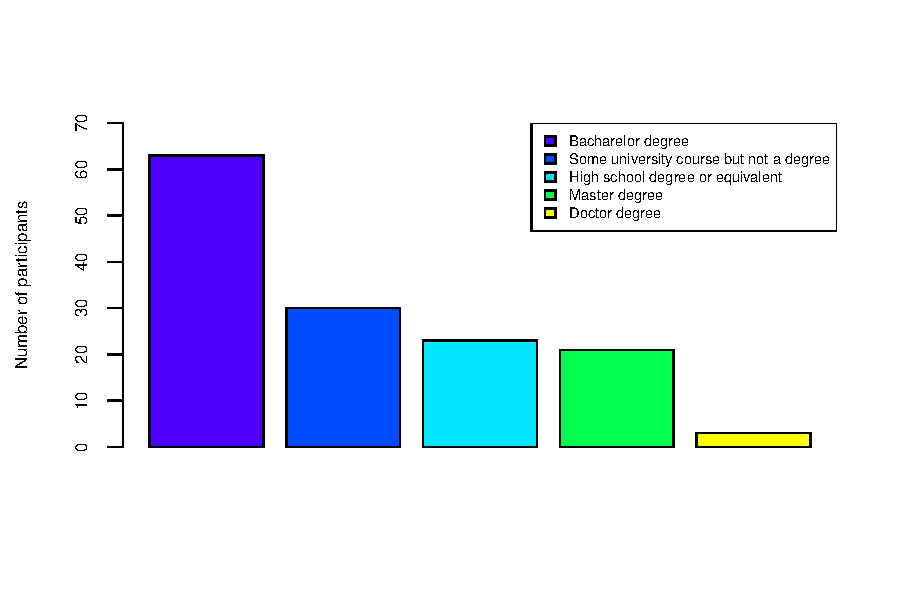
\includegraphics[width=\columnwidth]{images/dem-education-1.pdf}
%%       \caption{Participants' Education Level}\label{fig:degree}
%%   \end{figure}
  
%%   \begin{figure}[htb]
%%       \centering
%%       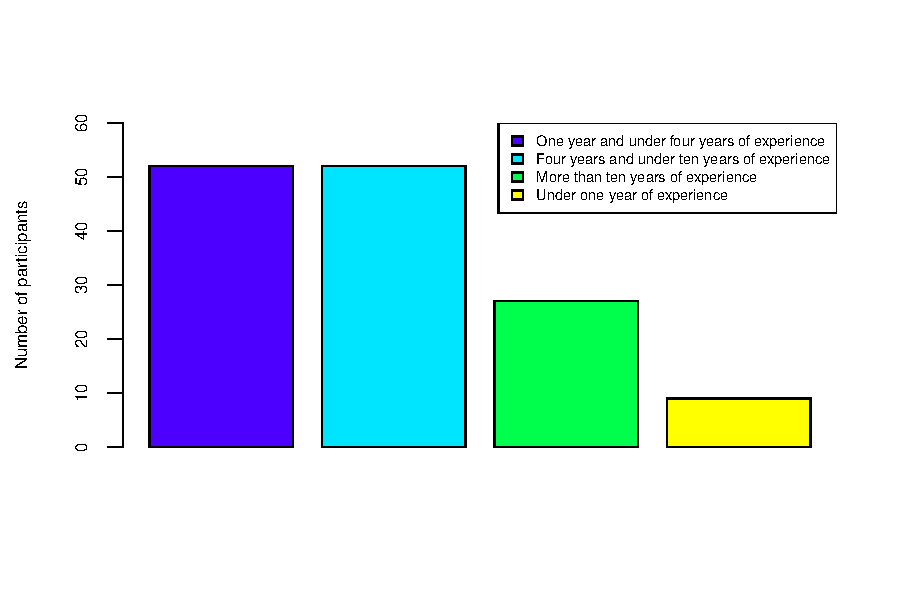
\includegraphics[width=\columnwidth]{images/dem-experience-1.pdf}
%%       \caption{Participants' Experience} \label{fig:xp}
%%   \end{figure}
%Figure~\ref{fig:xp} shows that more than a half of


\subsection{Misunderstanding Rate Analysis}

\subsubsection*{Exploratory Data Analysis}

As mentioned in Section~\ref{sec:meth:survey}, each participant in this study evaluated ten
code snippets, from which five were in their confusing versions, whilst the other five contained clean versions of the code snippets (i.e., without the confusing constructs and idioms). The participants should provide the expected outcomes of the code snippets. As discussed, we collected information about \emph{correctness} (whether the participant correctly predicted the program's output) and \emph{time}. 
Table~\ref{tab:difference-correctness} and Figure~\ref{fig:boxplotcorrectness} summarize the results of the survey w.r.t. correctness.

Considering Table~\ref{tab:difference-correctness}, the clean versions of six code snippets present at least a 15\% improvement in answer correctness when compared with the confusing versions. In particular, the presence of the \emph{Comma Operator} atom presents the highest impact on misunderstanding. 
Frequently used constructs and idioms, such as \emph{Post Increment} and \emph{Omitted Curly Braces} (see Section~\ref{sec:msr-results}), also result in many mistakes. %introduce high degrees of confusion.
The boxplot of Figure~\ref{fig:boxplotcorrectness} shows a non-negligible decrease in the average number of incorrect answers when observing the clean versions of the code snippets. Also, the sample of responses with no atoms had almost no dispersion, which supports the
argument that the non-confusing versions of the code snippets are easier to evaluate correctly. 


% \begin{table}[htbp]
% \caption{Difference in answer correctness between confusing and non-confusing pairs}
% \begin{center}
% \begin{small}
% \begin{tabularx}
% {{\linewidth}}{l p{1.5cm} p{1.1cm} p{1.1cm} p{1.2cm} }
% \textbf{Atom} & \textbf{\%Correct} & \textbf{\%Correct} \\
% &  \multicolumn{1}{l}{With AOC} \multicolumn{2}{l}{Without AOC}  & \Delta (\%)    \\
%  \hline
% Comma Operator & 40 & 93 & +132\%                 \\     
% Automatic Semicolon  Insertion & 46 & 97 & +110\% \\
% Post Increment & 69 & 91 & +31\%         \\
% Omitted Curly Braces & 67 & 83 & +23\%   \\ 
% Assignment as Value & 80 & 97 & +21\%    \\
% Implicit Predicate & 83 & 97 & +16\%     \\
% Logic as Control Flow & 59 & 68 & +15\%  \\
% Ternary Operator & 86 & 94 & +9\%        \\
% Pre-Increment & 71 & 76 & +7\%           \\
% Arithmetic as Logic & 91 & 90 & -1\%    \\
% \end{tabularx}
% \end{small}
% \end{center}
% \label{results_correctness}
% \end{table}

\begin{table}[htbp]
\caption{Summary of the correctness analysis}
\label{tab:difference-correctness}
\centering{
\begin{scriptsize}
\begin{tabular}{lccc} \toprule
  Atom & Confusing Code & Clean Code & $\Delta$(\%)  \\ \midrule
  Comma Operator                &  28 &  65 & +132   \\ 
  Automatic Semicolon Insertion &  32 &  68 & +112   \\ 
  Post-Increment                &  48 &  64 & +33    \\ 
  Omitted Curly Braces          &  47 &  58 &  +23   \\
  Assignment as Value           &  56 &  68 &  +21   \\ 
  Implicit Predicate            &  58 &  68 &  +17   \\ 
  Logic as Control Flow         &  41 &  48 &  +17   \\ 
  Ternary Operator              &  60 &  66 &  +10   \\ 
  Pre-Increment                 &  50 &  53 &  +6    \\ 
  Arithmetic as Logic           &  64 &  63 &  -2    \\ \bottomrule
  
\end{tabular}
\end{scriptsize}
}
\end{table}

 %% Comma Operator          & 40 & 93  & +132 \\
 %% Post Increment          & 69 & 91  & + 31  \\
 %% Omitted Curly Braces    & 67 & 83  & +23 \\
 %% Assignment as Value     & 80 & 97  & +21 \\
 %% Implicit Predicate      & 83 & 97  & +16 \\
 %% Logic as Control Flow   & 59 & 68  & +15 \\
 %% Ternary Operator        & 86 & 94  & +9  \\
 %% Pre-Increment           & 71 & 76  & +7  \\
 %% Arithmetic as Logic     & 91 & 90  & +1  \\ \bottomrule


\begin{figure}[b!]
\noindent
\vspace*{-1.4cm}
 \centering
 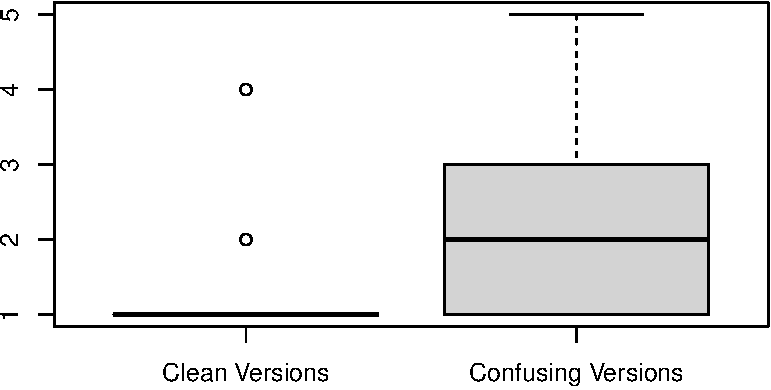
\includegraphics[width=\columnwidth]{images/wrong-answers-plot-1.pdf}
 \vspace*{-1.3cm}
 \caption{Number of wrong answers of each subject.}
 \label{fig:boxplotcorrectness}
 \end{figure}

% \rb{verificar a consistencia nas questoes de pesquisa mais especificas}

\subsubsection*{Hypothesis Testing and Effect Size}

We first use the \emph{Pearson's Chi-squared test}
to investigate if there is a statistically significant difference in the frequency of correct and incorrect answers---due to the versions of the code snippets (confusing and clean code). The p-values for these tests are reported in the ``Chi-square test'' column of Table~\ref{tab:hypothesis-testing}. The results indicate that for five atom candidates (Comma Operator, Automatic Semicolon Insertion, Post-Increment, Assignment as Value, Implicit Predicate) the confusing versions of the code snippets have a negative impact on code understanding (p-value $< 0.05$). This result holds even after applying the Benjamini-Hochberg correction with a false discovery rate of 5\%. 

We measure the effect size of the clean version of the code snippets into the answers' correctness using the \emph{Odds Ratio} (OR). The results are reported in the ``Odds Ratio'' column of Table~\ref{tab:hypothesis-testing}. In the table, we also report the confidence interval (CI) for the OR in the ``CI'' column. Although many of the intervals are wide, for six of the atom candidates the lower bound of the confidence interval is greater than or equal to 1. This indicates that, at a 95\% confidence level, a developer is likely to commit less mistakes when using the clean versions. 
%Considering only the atoms for which there was a significant difference in correctness for confusing and clean versions and u
Using the thresholds established by Chen and colleagues~\cite{Chen:2010:HBB} (OR = 1.68 small, 3.47 medium, and 6.71 large), for four of the atoms, Comma Operator, Automatic Semicolon Insertion, Assignment as Value, and Implicit Predicate, effect size can be considered large. For Implicit Predicate, it is medium. 
%We found a negligible effect size for the atom candidates Arithmetic as Logic, Logic as Control Flow, and Pre-Increment. Nonetheless, for the remaining candidates, the effect size is significant. 
For instance, when comparing clean and confusing code snippets pertaining to the Comma Operator atom candidate, we observed an \emph{Odds Ratio} of \num{19.02}. This means that the odds of a correct answer are \num{19.02} times higher when interpreting the clean version---in comparison with the corresponding confusing version of the code snippet. Furthermore, with a 95\% confidence level, the odds  ratio is between 6.6 and 68.22, i.e., although the error margin is wide, it is strongly in favor of the clean version. If there is a significant likelihood of a developer committing a mistake when analyzing a clean version, the lower bound of the CI should be a number between 0 and 1 (since the OR is a ratio). This is the case for the four atom candidates in the lower part of the table. In particular, in the last row (Arithmetic as Logic), the OR between 0 and 1 indicates that a participant was actually more likely to misunderstand the clean version. 

Finally, we also use the \emph{Binomial Generalized Logistic Regression} analysis to investigate if either participant \emph{education} or participant \emph{experience} impact correctness. Although the results suggest that experience impacts correctness, the education level does not. As such, we replicate the \emph{Pearson's Chi-squared test} for each experience group and found that the statistical difference is less significant for those developers with more than ten years of experience. 

\begin{mh}
  The results of our exploratory data analysis and   hypothesis testing suggest that the atom candidates Comma Operator, Automatic Semicolon Insertion, Post Increment, Omitted Curly Braces, Assignment as Value, and Implicit Predicate %, and Ternary Operator
  introduce some degree of misunderstanding in JavaScript code. %Based on the results of this study, 
  Therefore, they can be deemed atoms of confusion for JavaScript.
\end{mh}

%% Regarding the first question we 
%% address in the survey (\emph{Do code snippets that contain atoms of confusion produce a higher error rate than snippets where the atom is removed?}), we found evidence that the atoms of confusion lead programmers to misunderstand JavaScript code. We also realized that just one atom whose correction has a non-significant improvement in the percentage of correct answers---we found an improvement of at least 15\% in the correct answers when removing the confusing code for seven atoms (out of ten atoms we consider in the survey). 

\subsection{Time Analysis}

\subsubsection*{Exploratory Data Analysis}
Table \ref{tab:difference-time-taken} shows the average time necessary for the participants to give a correct answer about the expected outcomes of a code snippet, considering both confusing and clean versions. We do not consider cases where the participants made mistakes. Seven atom candidates required more time from participants to predict a correct response. For these seven atom candidates, developers take at least 5.90\% less time on average to find a correct answer when considering the clean version of a code snippet. In the extreme case (atom candidate Comma Operator), the participants take 76.23\% less
time on average to find the correct answer for the clean version of the code snippets. 
Not all atom candidates, though, require less time for the participants to predict the answer. In fact, for the Arithmetic as Logic and the Pre-Increment atoms, the time to give a correct answer increased  
29.06\% and 38.19\% for the clean versions.

\begin{table}[htbp]
\caption{Time in seconds to submit a correct answer}
\centering{
\begin{scriptsize}
\begin{tabular}{lccc} \toprule
Atom & Confusing Code & Clean Code & $\Delta$(\%) \\ \midrule
Comma Operator & 87.67 & 20.84 & -76.23 \\ 
Automatic Semicolon Insertion & 46.08 & 22.04 & -52.17 \\ 
Post-Increment & 28.70 & 25.67 & -10.56 \\ 
Omitted Curly Braces & 48.85 & 30.00 & -38.58 \\ 
Assignment as Value & 52.47 & 48.95 & -6.71 \\ 
Implicit Predicate & 36.24 & 24.01 & -33.75 \\ 
Logic as Control Flow & 108.94 & 51.07 & -53.12 \\ 
Ternary Operator & 41.80 & 39.34 & -5.90 \\ 
Pre-Increment & 30.71 & 42.45 & 38.19 \\  
Arithmetic as Logic & 28.82 & 37.20 & 29.06 \\ \bottomrule
\end{tabular}
\label{tab:difference-time-taken}
\end{scriptsize}
}
\end{table}

 % latex table generated in R 4.0.4 by xtable 1.8-4 package
 % Thu Apr 22 07:58:21 2021
 \begin{table*}[ht]
\caption{Hypotheses Testing (misunderstanding and time)}

 \centering
 \begin{tabular}{lccc|cc}
   \toprule
Atom  & Chi-square test & Odds Ratio          & CI & Mann-Whitey U test & Cliff's Delta \\ 
     &         & (misunderstanding)  &                    & (workload)             & \\ \midrule
Comma Operator & 1.1727e-10 & 19.02 & (6.60, 68.22) & 5.8249e-08 & -0.53 \\ 
Automatic Semicolon Insertion & 5.8352e-11 & 39.33 & (9.21, 356.62) & 0.09802 & -0.16 \\ 
Post-Increment & 0.0015279 & 4.83 & (1.73, 15.74) & 0.12006 & 0.15 \\ 
Omitted Curly Braces & 0.050962 & 2.35 & (1.00, 5.77) & 0.92529 & -0.01 \\ 
Assignment as Value & 0.0034775 & 8.39 & (1.81, 79.12) & 0.82681 & 0.02 \\ 
Implicit Predicate & 0.01123 & 6.95 & (1.46, 66.56) & 0.0029039 & -0.29 \\ 
Logic as Control Flow & 0.292 & 1.54 & (0.73, 3.28) & 7.5862e-05 & -0.39 \\ 
Ternary Operator & 0.15896 & 2.73 & (0.74, 12.57) & 0.24073 & -0.12 \\ 
Pre-Increment & 0.70147 & 1.25 & (0.55, 2.85) & 0.0062981 & 0.27 \\ 
Arithmetic as Logic & 1 & 0.84 & (0.22, 3.12) & 0.01723 & 0.23 \\ 
    \bottomrule
 \end{tabular}
 \label{tab:hypothesis-testing}
 \end{table*}


\subsubsection*{Hypothesis Testing}
We use the non-parametric \emph{Mann-Whitney U test}, also known as Wilcoxon rank-sum test, to
investigate the null hypothesis that developers 
spend the same amount of time to correctly
predict the outcome of a code snippet, regardless
of evaluating the confusing or clean version
of the code. The results of Table~\ref{tab:difference-time-taken}
suggests that we should refute the null hypotheses for five atom candidates (Comma Operator, Implicit Predicate, Logic as Control Flow, Pre-Increment, and Arithmetic as Logic), after applying the Benjamini-Hochberg correction with a false discovery rate of 5\%. For the first three, the analysis suggests that the participants need more time to predict the outcome of the code snippet in the confusing code version. For the atom candidates Arithmetic as Logic and Pre-Increment, the participants take less time to predict the outcome of the code snippets in the confusing version. We also computed the effect size using Cliff's Delta statistic. In the table, negative effect sizes suggest that it took less time to correctly predict the output of clean versions of the snippets.  Considering the thresholds established by Romano et al.~\cite{Romano:2006:ASO} (0.147 $<$ $|$d$|$ $<$ 0.33 small, $|$d$|$ $<$ 0.474 medium, otherwise large), we found a large effect for the Comma Operator atom candidate; a medium effect size for Logic as Control Flow, and small effect sizes for Automatic Semicolon Insertion, Implicit Predicate, Arithmetic as Logic, Post-, and Pre-Increment. 


\begin{mh}
  The results suggest that developers tend to spend
  more time to predict the correct answer in the presence of the atom candidates Comma Operator, Logic as Control Flow, and Implicit Predicate. Conversely, the code snippets with the atom candidates Arithmetic as Logic and Pre-Increment demand less time to predict the correct answers. 
\end{mh}


%%  Comma Operator        & 60 & 21  & -65  \\
%% Logic as Control Flow & 85 & 49  & -42  \\
%% Implicit Predicate    & 33 & 24  & -27  \\
%% Omitted Curly Braces  & 43 & 31  & -27  \\
%% Assignment as Value   & 53 & 49  & -7   \\
%% Ternary Operator      & 42 & 42  & 0    \\
%% Post Increment        & 27 & 27  & 0    \\
%% Arithmetic as Logic   & 29 & 36  & +24  \\
%% Pre-Increment         & 34 & 49  & +44  \\


\
% \rb{acho que podemos melhorar a apresenta\c c\~{a}o dessas tabelas, talvez usando booktabs.}

\vspace*{-0.5cm}
\section{Results of the Interview Study}
\label{sec:interview-results}

%% \rb{acho que essa separa\c c\~{a}o em dois rounds est\'{a}
%%   gerando uma complexidade desnecess\'{a}ria. vou tentar
%%   remover isso}.

In this section, we present the results of the 
interviews with the 15 practitioners who agreed to participate in the study. 
% A total of 15 practitioners took part of the interviews.
We collected information regarding programming
experience, familiarity with JavaScript, and their opinion about the \na atom candidates we explored in our research. We first presented them pairs of clean and confusing code snippets and then asked them to discuss their preferences towards one version. We did not indicate in any way whether any version was assumed to be confusing or not. 
% ask the participants to discuss their preferences (i.e., code with or without atom).


%% In the second round of interviews, ten of the fifteen developers
%% who participated in the first round were shown another 8 atom candidates to atom of confusion whose frequency we observed during the repository mining phase. The same procedure of showing code that behaves exactly the same and surveying for how easy to understand each snippet was applied in this phase. 

\begin{table}[!htb]
    \centering
    \caption{Summary of participants' preferences for code snippets \emph{with} and
      \emph{without} atom candidates. The participants were only presented the code snippets, without any indication about whether one was confusing or not. 
      Participants were also allowed to choose Neutral when they thought both sides were equally readable.}
    \begin{tabular}{lrrr}\toprule
      & \multicolumn{3}{c}{\textsc{Preference (\%)}} \\
      \cmidrule(lr){2-4}
         Atom           & \multicolumn{1}{c}{Confusing}
                                      &  \multicolumn{1}{c}{Clean}
                                               & \multicolumn{1}{c}{Neutral} \\ \midrule
         Comma Operator                  & 0  & 100    & 0     \\
         Automatic Semicolon Insertion  & 0  & 80     & 0     \\
         Post-Increment                  & 20 & 73.33  & 6.67  \\
         Omitted Curly Braces            & 0  & 100    & 0     \\
         Assignment as Value             & 20 & 60     & 20    \\
         Implicit Predicate              & 20 & 73.33  & 6.67  \\
         Logic as Control Flow           & 20 & 60     & 20    \\
         Ternary Operator                & 60 & 26.67  & 13.3  \\
         Pre-Increment                   & 40 & 46.67  & 13.33 \\ 
         Arithmetic as Logic             & 0  & 93.33  & 6.67  \\ \midrule
         \textsc{overall}                & 18 & 71.33  & 8.64  \\
         \bottomrule
    \end{tabular}
    \label{tab:interview-results1}
\end{table}

\subsubsection*{The Participants' perceptions of the atom candidates}
Supporting the results of the survey, Table~\ref{tab:interview-results1}
 shows that for eight out of the
10 scenarios surveyed, the majority of the respondents prefer the version of the
code without the atom candidate.
In no case the \emph{neutral}
ratio was higher than the option for the Clean version.
%% An example entry is contained in Appendix~\ref{}. 
%% For a full listing of the code snippets, visit the paper repository. 
Only for the Ternary Operator atom candidate the participants prefer the Confusing version, instead of the Clean one. We show the code snippets for the Ternary Operator in Figure~\ref{code:ternary}. Even for this atom candidate, some participants who preferred the left-hand side version (confusing) still believed that the right-hand side version (clean) was more readable. The following quotes were extracted from the transcripts with
% three interviewees:
two interviewees:

\begin{figure*}

\noindent\begin{minipage}{.45\textwidth}
\begin{lstlisting}[language=JavaScript, caption=\emph{Left-hand side} (using the \emph{Ternary Operator} atom).]
let config = {size: 3, isActive: false};
const_config = config.isActive === true 
             ? config 
             : {size: 10};
console.log(_config.size);
\end{lstlisting}
\end{minipage}\hfill
\begin{minipage}{.45\textwidth}
\begin{lstlisting}[language=JavaScript, caption=\emph{Right-hand side} (without the atom).]
let config = {size: 3, isActive: false}
let _config;
if(config.isActive === true) {
  _config = config;
}
else{
   _config = {size: 10};
}
console.log(_config.size);
\end{lstlisting}
\end{minipage}
\caption{Example of a pair of code snippets used in the interview. This case explores the use of the \emph{Ternary Operator atom of confusion}}
\label{code:ternary}
\vspace{-0.2cm}
\end{figure*}

\begin{mq}
\emph{``I prefer to write [code using the \lhs version], but I think [the \rhs version] is easier to read, especially for newer programmers''}.
\end{mq}

\begin{mq}
\emph{``When I am programming, I write code with the ternary operator, [...], but, to be honest, I still think that the 
[the code using the \rhs version] 
is easier to understand''}.
\end{mq}

%% \begin{mq}
%% \emph{``I think [the \lhs version] is easier to understand, but [the \rhs version] is what I would write"}
%% \end{mq}

%% The atom candidate Ternary Operator also opens up
%% the possibility for a derivative construct that JavaScript
%% allows which can be rather confusing, and that is the nested
%% ternaries construct, in which the right-hand side of the a
%% ternary operator can be another ternary construct.
%% While nested ternaries remove the number of lines that
%% would be necessary to construct using nested if-then-else statements,
%% they can become quite taxing to understand.
%% Nested ternaries are a choice of atoms to be analyzed in future work.

The Pre-Increment atom candidate also caused such
divide in one of the interviewees, who
regarded the clean version as simpler to understand, but would still opted to write
code with the atom. In contrast, %to such opinion,
one of the participants found the version with the atom candidate more elegant, but recognized it was less readable, and was willing to sacrifice elegance for readability.

%% \rb{pela discuss\~{a}o anterior, parece-me que alguns
%%   desenvolvedores reconhecem que esses candidatos
%%   a \'{a}tomos introduzem certa dificuldade de compreens\~{a}o;
%%   mas mesmo assim optam por usar a constru\c c\~{a}o correspondente.
%%   Acho que cabe um box aqui com essa discuss\~{a}o sobre isso.}

When analyzing the Logic as Control Flow atom candidate, one of the interviewees gave an example personal experience that might motivate one to avoid writing code using this construct:

\begin{mq}
  \emph{``This one is interesting, because I have written code that looks like the left-hand side [Confusing version], and my colleagues complained that it was difficult to understand. Nowadays I prefer to write code using the version on the right-hand side [Clean]''}.
\end{mq}

For two of the atom candidates, the interviewees were unanimous in their preference for the clean version: Comma Operator and Omitted Curly Braces. Regarding the first one, we could often notice during the interviews that the \emph{\lhs} (with the atom of confusion) caused significant confusion among the participants. One remark about the \emph{Comma Operator} atom of confusion is listed below:

%% \begin{mq}
%% \emph{``I just learned that [the \lhs version of this code] is possible. I did not even know it worked''}
%% \end{mq}

\begin{mq}
\emph{``The code in [the \lhs version] is unlikely to be understood unless the programmer knows \clang or \cpplang''}.
\end{mq}

As for the atom candidate Omitted Curly Braces, one of the interviewees mentioned that, although they understand why one would opt not to use braces for simple if-then-else statements, they still advised against it, on grounds that:

\begin{mq}
\emph{``[I prefer the \rhs version of the code \ldots]
If I want to see well-written, easily understandable code, then I also have to do my job. Therefore I believe that, since I do not know who is on the other end maintaining this code, and it could be any person with any level of expertise, then I try to write readable, easy-to-understand code''}.
\end{mq}

%This is an interesting perspective, because such a perhaps simple decision,  might hinder novice developers in the task of maintaining code; and one cannot make any assumption about the programmers' experience of who is going to maintain a code in a long run.

%This is an interesting perspective because such a simple decision might hinder novice developers in maintaining code; one cannot assume the programmers' experience of who will maintain a code in the long run.



\subsubsection*{Confusion in JavaScript Code} 

% The final remarks that were drawn from the interviews are related to potentially confusing constructs that were suggested by the participants, as well as their perspective on JavaScript as a language, from which we can also uncover some other forms in which the language itself might contribute to writing confusing code.

The final remarks drawn from the interviews are related to potentially confusing constructs suggested by the participants and their perspectives on JavaScript as a language. From the latter, we can also uncover some other forms in which the language itself might contribute to writing confusing code.

One of the participants mentioned that the use of JavaScript's prototype-based inheritance can make it difficult to understand code, particularly when involving deep prototype chains. This is a core feature of the language, and most high-level tools and frameworks abstract it away. Although this was only mentioned by one practitioner, this is an important remark, as true understanding of JavaScript software necessarily involves understanding the concept of prototypes.

% When asked about particular JavaScript constructs or patterns that can make code difficult to understand, three participants cited the callback pattern, which can lead to several levels of nested function calls, as extremely difficult to assimilate.
When asked about particular JavaScript constructs or patterns that can make code difficult to understand, three participants cited the callback pattern---potentially leading to several levels of nested function calls---as extremely difficult to assimilate. One of the respondents stated:

\begin{mq}
\emph{``Nested callbacks are very confusing. Even writing them can be confusing, let alone understanding them.''}
\end{mq}

Two other developers implicitly touched upon the callback pattern, mentioning that it can be difficult to understand \emph{asynchronous} programming in JavaScript. Since what is really happening at a lower level is that the JavaScript engine creates a callback stack that is separate from the main execution stack, and that callback functions are only executed when the main execution stack is empty, the concepts of asynchronous events and callbacks are inseparable in the language, and any abstractions for callback functions, such as promises and async/await syntax only hide the pattern. We also found other idioms that are JavaScript atom candidates, including
\emph{property access} via array subscription (\lstinline[language=javascript]{V1['P1']} instead of \lstinline[language=javascript]{V1.P1}) and \emph{arrow functions} (see listings~\ref{arr1} and~\ref{arr2}). 

\begin{figure}
\begin{small}
\begin{lstlisting}[language=JavaScript,caption=Example of arrow function.,label=arr1]
let inc = (x) => x + 1;
\end{lstlisting}
\begin{lstlisting}[language=JavaScript,caption=Alternative version without arrow function.,label=arr2]
let inc = function(x) {
  return x + 1
}
\end{lstlisting}
\vspace*{-0.6cm}
\end{small}
\end{figure}

% citar uninitialized objects' types. floating point precision issues, 'this', type coercion

% \subsection{Common Misunderstandings About the Language}

% TODO: I don't see that our results support these claims.
% Let us comment for now.

%% Six practitioners regarded the JavaScript language as easy to learn, while four
%% participants mentioned that the abundance of frameworks,
%% coupled with the abstractions they provide, make it so that one
%% can develop quickly in the language. However, as mentioned by one
%% of the interviewees, ``\emph{Developers who have started
%% programming in JavaScript might miss out on important lower-level
%% aspects, such as garbage collection, memory management,
%% and process management.}''. 

%% Moreover, such abstractions might lead a developer to start to program
%% using the language without actually understanding some of its basic aspects.
%% For instance, four participants argued that the language is not typed, two  believed the language runs exclusively on browsers, and two other developers stated that the language is natively asynchronous, all of which are incorrect statements.
%% For the multi-purpose language that is one of the most, if not the most used one by practitioners,
%% a lack of understanding of the languages core
%% features may be a problem worth investigating in future studies.



%% \begin{table}[!htb]
%%     \centering
%%     \caption{Interviews Round 2 - Summary of participants' preferences for code snippets \textsc{with} and \textsc{without} atoms of confusion (\textsc{aoc}). Participants were also allowed to choose \textsc{neutral} when they thought both sides were equally readable.}
%%     \label{tab:interview-results2}
%%     \begin{tabular}{lrrr}\toprule
%%       & \multicolumn{3}{c}{\textsc{Preference (\%)}} \\
%%       \cmidrule(lr){2-4}
%%          \textsc{atom}           & \multicolumn{1}{c}{\textsc{with aoc}}
%%                                       &  \multicolumn{1}{c}{\textsc{without aoc}}
%%                                                & \multicolumn{1}{c}{\textsc{neutral}} \\ \midrule
%%          Property access         & 10  & 60  & 30  \\
%%          Object spread           & 50 & 50     & 0    \\
%%          Array spread            & 60  & 40    & 0     \\
%%          Arrow function          & 40 & 40     & 20  \\
%%          Array destructuring     & 40 & 40  & 20  \\
%%          Object destructuring    & 40 & 40     & 20    \\
%%          Type conversion         & 30  & 60    & 10     \\
%%          Change Literal encoding & 40 & 50  & 10  \\ \midrule
%%          \textsc{overall}        & 42.8 & 47.6  & 9.6  \\
%%          \bottomrule
%%     \end{tabular}
%% \end{table}

\section{Results of the MSR Effort}
\label{sec:msr-results} 

We mined \minedprojects open source JavaScript repositories to understand how
often atoms of confusion arise in real software. 
Similarly to previous studies~\cite{DBLP:conf/msr/GopsteinZFC18,DBLP:journals/ese/MedeirosLAAKRG19}, which investigate
the prevalence of atoms of confusion in open source \clang and \cpplang projects, we found that atoms of confusion
frequently arise in JavaScript open source systems. For instance, the six most frequently found atoms
occur in at least 80\% of the projects. Considering the extremes, atom candidates Ternary Operator and Implicit Predicate were found in all repositories we mined,
while Comma Operator occurred in only 15\% of them (as seen in Table~\ref{tab:occurrences-summary}).

% Figure~\ref{fig:rate} summarizes this finding, showing that the occurrence of atoms of confusion in JavaScript systems range from 11.34\% (Comma Operator) to 89.69\% (Ternary Operator).


%Figure~\ref{fig:atoms-occurrence} shows that the occurrence of in JavaScript systems range from 

% latex table generated in R 4.0.3 by xtable 1.8-4 package
% Fri Nov 13 11:28:56 2020
%%\begin{table}[!htb]
%%\centering
%% \caption{Summary of atoms occurrences on our dataset}
%% 
%%\setlength\tabcolsep{2pt} % default value: 6pt
%%\label{tab:occurrences-summary}
%%\begin{tabular}{lrcc}
%%
%%  \hline
%%Atom & Projects & Occurrences/KLOC & Category \\ 
%% \hline
%%Ternary Operator & 100\% & 10.16 &  highly used \\ 
%%Omitted Curly Braces & 91.67\% & 6.61 &  highly used \\ 
%%Post Increment & 90.28\% & 5.62 &  highly used \\ 
%%Pre-Increment & 83.33\% & 1.04 & commonly used \\ 
%%Assignment as Value & 81.94\% & 1.02 & commonly used \\ 
%%Logic as Control Flow & 56.94\% & 0.95 & commonly used \\ 
%%Arithmetic as Logic & 23.61\% & 0.02 & little used \\ 
%%Comma Operator & 15.28\% & 0.03 & little used \\ 
%%   \hline
%%\end{tabular}
%%\end{table}

% latex table generated in R 4.0.3 by xtable 1.8-4 package
% Tue Apr 13 09:34:35 2021
\begin{table}[ht]
\centering
\caption{Summary of atom candidate occurrences on our dataset.}
\setlength\tabcolsep{2pt} % default value: 6pt
\begin{tabular}{lrc}%c}
  \toprule
Atom & Projects & Occurr./KLOC \\%& Frequency \\ 
  \midrule
Implicit Predicate & 100\% & 19.89 \\%&  intensively used \\ 
  Ternary Operator & 100\% & 10.16 \\%&  intensively used \\ 
  Omitted Curly Braces & 91.67\% & 6.61 \\%&  intensively used \\ 
  Post Increment & 90.28\% & 5.62 \\%&  intensively used \\ 
  Pre Increment & 83.33\% & 1.04 \\%& commonly used \\ 
  Assignment as Value & 81.94\% & 1.02 \\%& commonly used \\ 
  Logic as Control Flow & 56.94\% & 0.95 \\%& commonly used \\ 
  Automatic Semicolon Insertion & 33.33\% & 0.13 \\%& commonly used \\ 
  Arithmetic as Logic & 23.61\% & 0.02 \\%& rarely used \\ 
  Comma Operator & 15.28\% & 0.03 \\%& rarely used \\
   \bottomrule
\end{tabular}
\label{tab:occurrences-summary}
\end{table}


Considering all JavaScript projects in our dataset, we found a total of \num{364873} atom candidates, though four atoms are responsible
for 92.97\% of this total: Implicit Predicate, Post Increment, Ternary Operator, and Omitted Curly Braces. The first two, based on the results of Section~\ref{sec:survey-resuts}, can be considered atoms of confusion. The remaining atom
candidates comprise \num{25621} occurrences combined, 7.03\% of the total number of occurrences.
The Comma Operator and Arithmetic as Logic atoms are the ones that arise less
frequently (0.001\% in total with 232 and 165 occurrences, respectively). 

% Regarding frequency, we proceeded with a classification of \emph{atom occurrence}
% based on thresholds used in a previous
% study~\cite{DBLP:journals/ese/MedeirosLAAKRG19}. 
% Atoms that occur 1000 times are classified as \textit{rarely used} while atoms with more than \num{10000} occurrences are classified as \textit{highly used}; \textit{commonly used} atoms occur in between.
We calculated the frequency of each atom per KLOC.
The four atoms mentioned in the previous paragraph,
 Implicit Predicate, Post Increment, Ternary Operator, and Omitted Curly Braces, occur frequently in the analyzed projects. All of them have more than 5 occurrences per KLOC on average. In particular, two atom candidates occur very frequently, Implicit Predicate (19.89 occurrences per KLOC) and Ternary Operator (10.16 occurrences per KLOC). On the other hand, Arithmetic as Logic and Comma Operator occur less than once for every 50 KLOC. 

%In our dataset of JavaScript projects, 
%We found the Ternary Operator atom occurring more frequently than the Omitted Curly Braces, differently from what has been reported in a previous work~\cite{DBLP:conf/msr/GopsteinZFC18}. %

The results of our survey and interviews suggest that the Ternary Operator does not contribute significantly as a source of misunderstanding (increasing the number of wrong answers in 9\% of the cases, according to our survey). Nonetheless, the Post-Increment Expression and Automatic Semicolon Insertion atoms are listed in the top four sources of misunderstanding  (Table~\ref{tab:difference-correctness}), and also frequently appear in open source systems. As such, fixing the the Post-Increment and Automatic Semicolon Insertion might improve the readabiliy of large amounts of code in JavaScript projects. 

\section{Discussion}
\label{sec:discussion}

\castor{Which atoms? The weight of experience. Statistical significance vs. practical relevance. Most of them, with the exception of Comma Operator and Object Destructuring, have also been observed for Java programs~\cite{Langhout:2021:ACJ}.

In addition, many of the coding idioms that have been previously identified as atoms of confusion in previous work~\cite{DBLP:conf/sigsoft/GopsteinIYDZYC17,Langhout:2021:ACJ}, such as Logic as Control Flow

Differences among the two studies, for example, post increment was not significant in the first one but it was significant in the second.
}

Our work has several implications.
First, it adds external validity to the
work of Gopstein et al.~\cite{DBLP:conf/sigsoft/GopsteinIYDZYC17},
which investigates
the impact of atom candidates on
understanding \clang,\cpplang code. That is,
similarly to their work, the atom candidates
Comma Operator, Post/Pre Increment, Omitted Curly Braces,
Assignment as Value, Implicit Predicate, and Logic as
Control Flow seem to make 
JavaScript code harder to understand. For five of them, the difference is statistically significant, with a large effect size for four atoms. Our results also 
refute the hypothesis that Arithmetic as Logic is an atom of confusion (i.e., a source of misunderstanding).
In comparison to the original
work of Gopstein et al.~\cite{DBLP:conf/sigsoft/GopsteinIYDZYC17}, 
our study
led to some differences in the effect size
of the atom candidates.
Altogether, we answer our first research question.

\begin{mh}
  {\bf Answer to RQ1:} The first study (survey) gives evidence that some of the atom candidates in \clang and \cpplang programs that also exist in JavaScript correspond to a source of misunderstanding in
  JavaScript code. 
\end{mh}

The results of the interview study complement the understanding of atoms of confusion because the participants make clear the existence of a trade-off between code comprehension and other quality attributes. For instance, most of the participants prefer the version of the code with the Conditional Operator, even though they agree that its use might contribute to the misunderstanding of JavaScript code, particularly when novices are maintaining the codebase. The participants of the interview study also
mentioned other possible sources of misunderstanding in JavaScript,
including the use of prototype-based inheritance and nested call-backs (as discussed in Section~\ref{sec:interview-results}). Other JavaScript atom candidates include
Object Destructuring, Array Spread, Object Spread, and Type Conversion.
In summary, the results of the second study (interviews) allow
us to answer the second research question.

\begin{mh}
  {\bf Answer to RQ2:} The qualitative analysis of the
  interviews supports the results of the first study,
  since JavaScript developers most often agree that atoms of confusion compromise
  source code understanding. 
\end{mh}

%% \begin{mh}
%%   {\bf Answer to RQ3:} The qualitative analysis of the
%%   interviews suggests that specific JavaScript constructs might also correspond to atoms of
%%   confusion, including prototype inheritance and
%%   nested callbacks. 
%% \end{mh}

The results of the third study (mining open source
JavaScript repositories) provides evidence that,
although atoms of confusion compromise program
comprehension, they frequently appear in open
source JavaScript projects. In particular,
seven, out of 10 atoms considered
  in our study, appear in more than 50\% of
the 72 projects we analyzed. Furthermore, at least two of them are used intensively, more than once for every 200 lines of code. In summary, the third study
allows us to answer the third research
question.


\begin{mh}
  {\bf Answer to RQ3:} The MSR study reveals that
  the several atom candidates explored in our research
  appear frequently in practice, and cleaning up the use of 
  Post-Increment/Decrement and the Automatic Semicolon Insertion
  might improve the readabiliy of JavaScript code substantially. 
\end{mh}



%% We conducted a non-exact replication of the three
%% studies (survey, interview, and mining software repositories)
%% considering these more specific JavaScript atom candidates.
%% We confirmed that they truly correspond to sources of misunderstanding.
%% Due to lack of space,
%% we cannot present all the results here, and we postpone the presentation of these results as future work.




\section{Threats to Validity}
\label{threat}

%Conclusion validity is connected with how well it is possible to establish relationships between treatments and outcomes. Threats to conclusion validity often come from inappropriate use of statistics. 

\textbf{Conclusion validity.} In the context of our survey study, we apply different statistical tests appropriate for the cases where data was categorical (correctness, Chi-square test of independence) and continuous (time, Mann-Whitney U test). Furthermore, besides reporting p-values, we also report effect size measures appropriate for each scenario (odds-ratio and Cliff's delta) and apply a p-value correction technique to avoid the multiple testing problem. Finally, it could be argued that the size of the samples is insufficient to make conclusions for some of the atoms, a common problem in Empirical Software Engineering. We estimate the sample size for each one of the atom candidates, considering that each one had a different number of samples (Table~\ref{tab:difference-correctness}). To that end, we use the $\phi$ measure of effect size for each atom (based on the Chi-square statistic), the standard $\alpha$ coefficient of 0.05, and set the expected statistical power to 0.8, as usually employed in the literature~\cite{Ellis:2010:EGE}. As a result of this analysis, we discover that for all but one of the atoms where we had a statistically significant result for correctness, Implicit Predicate, the sample size is sufficient. For the ones where we did not find statistically significant results for correctness, in fact the sample sizes we have analyzed are insufficient for such small effect sizes. This indicates that further studies on these atoms are required, due to the likelihood of type II errors.

%One threat to validity we have not properly addressed is lack of power, a common problem in Software Engineering research. 

%Construct validity is connected with how well the selected measures actually represent the concept of interest. 

\textbf{Construct validity.} We use correctness as a proxy for program comprehension. Furthermore, we use predicted outcomes of small programs as a measure of correctness. As discussed elsewhere~\cite{Oliveira:2020:ECR}, this approach is a test of the developers' ability to trace programs. Although this is a common approach in studies about atoms of confusion~\cite{TheEyesDoNotLie,Langhout:2021:ACJ,DBLP:conf/sigsoft/GopsteinIYDZYC17}, other measures of correctness could have been employed, potentially yielding different results. As a complement to correctness in the survey, we have measured the time it took for the participants to correctly predict the outcome of the code snippets (either with or without atom candidates). Furthermore, we have  asked the interviewees about their preferences when comparing confusing and clean versions of the programs.

%A potential problem with our method is that there little incentive for subjects to think thoroughly about the questions. We observed a lack of engagement when we ran the survey with undergraduate students during a pilot study. Although our final subjects were voluntarily partaking in the survey, we could not be sure that, after some time taking the survey, respondents would become tired and stop thinking clearly about the code.


%Internal validity is concerned with how well the study isolates the variables of interest and accounts for confounding factors. 

\textbf{Internal validity.} Since the survey was conducted online with unknown participants, we have no way of confirming their levels of education and experience. We mitigate this threat by, in the data analysis, explicitly accounting for programmer experience and using an experimental design that allows us to isolate the impact of the treatment from factors such as experience and formal education level. Also, we did not have a way to prevent respondents from cheating, such as running the code on an interpreter, or consulting other people. We partially mitigate this threat by presenting images with source code, instead of text. This creates an obstacle for participants to run the code while taking the survey.

%External validity is linked to whether it is possible to extrapolate the results of the study. 

\textbf{External validity.} Although our results suggest that the selected idioms and code constructs may lead to confusion for small code snippets, it is not clear whether that result extrapolates to other scenarios. Even though it is likely that in larger code bases the confusion induced by these constructs may be even greater, the existence of additional context may mitigate this effect. Another possible threat to the generalizability of our results, in particular for the survey and interviews, lies in the fact that the analyzed atoms may rarely occur in real JavaScript code bases. To mitigate that threat, we have analyzed 72 popular open source JavaScript repositories and found out that most of them are common, occurring at least once per 1,000 lines of code. Only Arithmetic as Logic and Comma Operator occur less frequently than once per 10,000 lines of code. 
\castor{A forma como os átomos foram detectados é uma ameaça que não discutimos.}


%% Finally, in one of the atoms, namely the Omitted Curly Braces,
%% we intentionally removed indentation from the original code,
%% which is highly unusual, given that many programmers use automatic
%% formatting in their code editors. This can introduce some level
%% of artificiality to this atom's question. Nonetheless,
%% we discovered that JavaScript does allow the programmer
%% to omit the curly braces after \textit{if} statements,
%% and insert multiple statements in the following line.
%% This fact itself might constitute
%% a source of confusion, which we leave to analyse
%% in our future endeavors. 

\section{Conclusions}
\label{conclusion}

\rb{draft. apenas movi esse texto que estava em settings para ca. pode servir de inspiracao para responder algumas das questoes de pesquisa.}

{\color{blue}Based on these results, we provide evidence that, although the atoms of confusion considered in our study do not take a much higher amount of time to predict the output of the code, their impact on program comprehension is, in almost all of our cases, highly significant.}
% \section{Atoms of Confusion Considered in our Research}\label{sec:appendix-atoms} 

\begin{atom}{Arithmetic as Logic}
\emph{Use of the result of an arithmetic expression as control logic.}

\begin{lstlisting}[language=JavaScript]
if(array_1.length - array_2.length){
  console.log(true);
}
\end{lstlisting}
\end{atom}

\todo[inline]{detalhar os demais atomos seguindo esse padr\~{a}o}

\begin{longtable}{| p{.50\linewidth} | p{.50\linewidth} |} 
% \begin{center}
\caption*{Code Snippets presented on the survey}
% \begin{tabular}{ | p{8.2cm} | p{8.2cm} | } \hline

\hline
\multicolumn{2}{| c |}{Arithmetic as Logic}  \\ \hline
Obfuscated ID: 11  Obfuscated Answer: false  &  Transformed ID: 1  Transformed Answer: false \\ \hline
\begin{lstlisting}[language=JavaScript]
let array_1 = [1,2,3];
let array_2 = [2,3,2];
if(array_1.length - array_2.length){
  console.log(true);
}
else{
  console.log(false);
} \end{lstlisting}
& 
\begin{lstlisting}[language=JavaScript]
let array_1 = [1,2,3];
let array_2 = [2,3,2];
if(array_1.length != array_2.length){
  console.log(true);
}
else{
  console.log(false);
} \end{lstlisting} \\ \hline


\multicolumn{2}{| c |}{Assignment as value}  \\ \hline
Obfuscated ID: 12  Obfuscated Answer: 0  &  Transformed ID: 2  Transformed Answer: 0 \\ \hline
\begin{lstlisting}[language=JavaScript]
function resetSchedulerState () {
  let activatedChildren = {length: 10};
  let index = length = activatedChildren.length = 0;
  console.log(index);
}
resetSchedulerState(); \end{lstlisting}
& 
\begin{lstlisting}[language=JavaScript]
function resetSchedulerState () {
  let activatedChildren = {length: 10};
  activatedChildren.length = 0;
  let length = activatedChildren.length;
  let index = length;
  console.log(index);
}
resetSchedulerState(); \end{lstlisting} \\ \hline


\pagebreak 
\hline
\multicolumn{2}{| c |}{Automatic Semicolon Insertion}  \\ \hline
Obfuscated ID: 13  Obfuscated Answer: false  &  Transformed ID: 3  Transformed Answer: true \\ \hline
\begin{lstlisting}[language=JavaScript]
function example(){
  return
      10
}
if(example() == 10){
  console.log(true);
}
else{
  console.log(false);
} \end{lstlisting}
& 
\begin{lstlisting}[language=JavaScript]
function example(){
  return 10;
}
if(example() == 10){
  console.log(true);
}
else{
  console.log(false);
} \end{lstlisting} \\ \hline


\multicolumn{2}{| c |}{Comma Operator}  \\ \hline
Obfuscated ID: 14 Obfuscated Answer: 13  &Transformed ID: 4 Transformed Answer: 3 \\ \hline
\begin{lstlisting}[language=JavaScript]
let V1 = 5, V2 = 10;
V1 = (V2 = 1, 2);
console.log(V1+V2);
\end{lstlisting}
& 
\begin{lstlisting}[language=JavaScript]
let V1 = 5, V2 = 10;
V2 = 1;
V1 = 2;
console.log(V1+V2);
\end{lstlisting} \\ \hline

\pagebreak
\hline
\multicolumn{2}{| c |}{Ternary Operator}  \\ \hline
Obfuscated ID: 15 Obfuscated Answer: 10  &Transformed ID: 5 Transformed Answer: 10 \\ \hline
\begin{lstlisting}[language=JavaScript]
let config = {size: 3, isActive: false};
const _config = config.isActive === true ? config : {size: 10};
console.log(_config.size); \end{lstlisting}
& 
\begin{lstlisting}[language=JavaScript]
let config = {size: 3, isActive: false}
let _config;
if(config.isActive === true){
  _config = config;
}
else{
  _config = {size: 10};
}
console.log(_config.size); \end{lstlisting} \\ \hline




\multicolumn{2}{| c |}{Implicit Predicate}  \\ \hline
Obfuscated ID: 16 Obfuscated Answer: false&Transformed ID: 6 Transformed Answer: false \\ \hline
\begin{lstlisting}[language=JavaScript]
let V1 = 10, V2 = 3;
if (!(V1 % V2)){
  console.log(true);
}
else{
  console.log(false);
} \end{lstlisting}
& 
\begin{lstlisting}[language=JavaScript]
let V1 = 1, V2 = 2;
if ((V2 - V1) == 0){
  console.log(true);
}
else{
  console.log(false);
} \end{lstlisting} \\ \hline





\multicolumn{2}{| c |}{Logic Control Flow}  \\ \hline
Obfuscated ID: 17 Obfuscated Answer: 7&Transformed ID: 7 Transformed Answer: 21 \\ \hline
\begin{lstlisting}[language=JavaScript]
let V1 = 3;
let V2 = 5;
let V3 = 0;
while (V1 != V2 && ++V1) {
  V3++;
}
console.log(V1 + V3); \end{lstlisting}
& 
\begin{lstlisting}[language=JavaScript]
let V1 = 1;
let V2 = 11;
let V3 = 0;
while (V1 != V2) {
  V1++;
  V3++;
}
console.log(V1+V3); \end{lstlisting} \\ \hline



\multicolumn{2}{| c |}{Omitted Curly Braces \& Indentation}  \\ \hline
Obfuscated ID: 18 Obfuscated Answer: 4  &Transformed ID: 8 Transformed Answer: 4 \\ \hline
\begin{lstlisting}[language=JavaScript]
let V1 = 1, V2 = 2
if (V1 > V2)
V2 = 1
V1 = 2
console.log(V2+V1) \end{lstlisting}
& 
\begin{lstlisting}[language=JavaScript]
let V1 = 1, V2 = 2;
if (V1 > V2) {
  V2 = 1;
}
V1 = 2;
console.log(V2+V1); \end{lstlisting} \\ \hline



\multicolumn{2}{| c |}{Post Increment}  \\ \hline
Obfuscated ID: 19 Obfuscated Answer: true&Transformed ID: 9 Transformed Answer: true\\ \hline
\begin{lstlisting}[language=JavaScript]
let V1 = 0;
if (V1++ == 0) {
  console.log(true);
}
else {
  console.log(false);
} \end{lstlisting}
& 
\begin{lstlisting}[language=JavaScript]
let V1 = 0;
if (V1 == 0) {
  console.log(true);
}
else {
  console.log(false);
}
V1 = V1 + 1; \end{lstlisting} \\ \hline



\multicolumn{2}{| c |}{Pre Increment}  \\ \hline
Obfuscated ID: 20  Obfuscated Answer: 2  &  Transformed ID: 10  Transformed Answer: 1 \\ \hline
\begin{lstlisting}[language=JavaScript]
var index = 1;
while (++index < 10) {
  console.log(index);
  break;
} \end{lstlisting}
& 
\begin{lstlisting}[language=JavaScript]
var index = 0;
index = index + 1;
while (index < 10) {
  console.log(index);
  index = index + 1;
  break;
} \end{lstlisting} \\ \hline



% \end{tabular}
% \end{center}
% \end{table}
\end{longtable}


% \section*{Acknowledgment}

\bibliographystyle{IEEEtran}
\bibliography{reference}

\vspace{12pt}
\end{document}
